\documentclass{article}

\usepackage[letterpaper, margin=1in, footskip=0.25in]{geometry}
\usepackage{fancyhdr}
\usepackage{amsmath}
\usepackage{graphicx}
\usepackage{wrapfig}
\usepackage{csquotes}
\usepackage{subcaption}
\usepackage{amssymb}
\usepackage{commath}

\MakeOuterQuote{"}

\newcounter{example}% Counter
\newcommand{\ex}{\stepcounter{example} \paragraph{Example \theexample}}

\title{Classifying One-variable Functions by Integrability}
\author{Steven Labalme}
\date{\today}

\begin{document}




\pagenumbering{gobble}
\maketitle
\newpage

\pagenumbering{roman}
\tableofcontents
\listoffigures
\listoftables
\newpage

\pagenumbering{arabic}
\pagestyle{fancy}
\fancyhf{}
\rfoot{Labalme \thepage}
\renewcommand{\headrulewidth}{0pt}

\setcounter{secnumdepth}{0}
\begin{center}
\section{Abstract}
\end{center}
The purpose of this paper is to separate the various functions explored at the Calculus I-II level by their techniques of integration. Integral calculus is roughly one-half of Calculus, so it is important to understand how to integrate a wide variety of functions, especially since techniques vary from the one-step application of rules of integration to complicated approximations. This report should provide a detailed analysis of various functions that can be used by people new to integration as well as returning players. It could be used as a supplemental reading to reinforce ideas and/or cast them in a different light.\par
An example-solution strategy is taken to convey the differences in integrability. For time's sake, only one function of each type (18 types, total) is explored. The reasons that past methods do not work are often briefly explored at the beginning of each example. However, it is more generally left to the reader to be able to classify a function that they may be faced with into one of the categories listed.
\newpage



\setcounter{secnumdepth}{3}
\section{Algebraically Integrable Functions}
\subsection{Functions of \emph{x}}
\subsubsection{Simple}
\paragraph{Introduction} It is simplest to integrate functions such as those in this section via antiderivatives. Integration of these functions generally requires rules of integration directly derived from rules of differentiation without a great deal of manipulation beforehand. Therefore, it is a logical starting place for this exploration of the different techniques of integration.
\ex This example is concerned with integrating the following function.$$y=3x^2+2x+1$$This can be accomplished with two rules of integration --- the sum and difference rule, and the antipower rule. The sum and difference rule states that the integral of the sum or difference of two functions can be evaluated as the integral of the two functions separately. Symbolically,$$\int_a^b (f(x)\pm g(x))\, dx=\int_a^b f(x)\, dx\pm\int_a^b g(x)\, dx$$The antipower rule states that the integral of a coefficient times a variable to a power is the coefficient divided by the original power plus one times the variable to the power of the original power plus one. Symbolically,$$\int_a^b kx^n\, dx=\left[\frac{kx^{n+1}}{n+1}\right]_a^b$$\par
Let's begin integrating. Write the integrable equation as follows.
\begin{equation*}
    y=\int (3x^2+2x+1)\, dx
\end{equation*}
Employ the sum and difference rule twice.
\begin{equation*}
    y=\int 3x^2\, dx+\int 2x\, dx+\int 1\, dx
\end{equation*}
Employ the antipower rule three times.
\begin{equation*}
    y=\left[\frac{3x^{2+1}}{2+1}\right]+\left[\frac{2x^{1+1}}{1+1}\right]+\left[\frac{1x^{0+1}}{0+1}\right]
\end{equation*}
Simplify and add the constant of integration to yield the following, final integrated equation (equation 1).
\begin{equation}
    y=x^3+x^2+x+C
\end{equation}
\ex This example is concerned with integrating the following function.$$y=x^{-1}$$This is a deceptively complicated problem. At first glance, it seems like the antipower rule is the simple solution, but employing it (as follows) would require dividing by zero.
\begin{align*}
    y &= \int x^{-1}\, dx\\
      &= \left[\frac{x^{-1+1}}{-1+1}\right]\\
      &= \frac{x^0}{0}\\
      &= \frac{1}{0}
\end{align*}
Instead, the solution requires a new rule of integration --- that the integral of the differential of a variable over that variable is the natural log of the absolute value of that variable. Symbolically,$$\int_a^b \frac{dx}{x}=\left[\ln|x|\right]_a^b$$A short proof follows (note that the absolute value of $x$ is added in at the end to extend the domain of the integral).\par
\begin{align*}
    y &= \ln x\\
    \text{e}^y &= x\\
    \frac{d}{dx}\left(\text{e}^y\right) &= \frac{d}{dx}\left(x\right)\\
    \text{e}^y\frac{dy}{dx} &= 1\\
    \frac{dy}{dx} &= \frac{1}{\text{e}^y}\\
    \frac{dy}{dx} &= \frac{1}{x}\\
    dy &= \frac{1}{x}\, dx\\
    \int dy &= \int \frac{1}{x}\, dx\\
    y &= \int \frac{dx}{x}\\
    \ln x &= \int \frac{dx}{x}\\
    \ln |x| &= \int \frac{dx}{x}
\end{align*}\par
Let's begin integrating. Write the integrable equation as follows.
\begin{equation*}
    y=\int x^{-1}\, dx
\end{equation*}
Employ the definition of negative exponents.
\begin{equation*}
    y=\int \frac{1}{x}\, dx
\end{equation*}
Multiply fractions.
\begin{equation*}
    y=\int \frac{dx}{x}
\end{equation*}
Simplify and add the constant of integration to yield the following, final integrated equation (equation 2).
\begin{equation}
    y=\ln |x|+C
\end{equation}
\paragraph{Summary} As Examples 1 and 2 have shown, polynomial functions of $x$ can be integrated via rules directly related to the sum and difference and power rule of derivatives as well as the fact that $\text{e}^x$ is its own derivative. The functions subsequently explored in Section 1.1.2 cannot be integrated with altered derivative rules and require some algebraic manipulation to transform them into such a state.
\newpage

\subsubsection{Advanced Algebraic Techniques}
\paragraph{Introduction} Though some functions, as seen in the previous section, are readily integrable using rules of integration, others need some algebraic manipulation before such rules can be employed. The functions in this section are deceptively simple when first looking at them, but yet they require some inspired techniques to transform them into such a state that one of the rules from the previous section can be used. However, for the purposes of this section, all algebraic manipulation can be fully understood by someone who has not studied calculus.
\ex This example is concerned with integrating the following function.$$y=\csc(x)$$Many trigonometric functions have integrals consisting of a trigonometric expression within the natural log function i.e. they are derived by manipulating the function into the form of derivative over function, or$$\frac{dv}{v}$$For example, to take the integral of $\cot(x)$, transform it into$$\frac{\cos(x)}{\sin(x)}$$which, according to the rule used in Example 2, is equal to$$\ln|\sin(x)|+C$$when integrated if $u=\sin(x)$ and $du=\cos(x)\, dx$.\par
However, some functions, like the cosecant function which is the focus of this example, require more algebraic work than the recognition of an alternate form of the function ($\frac{1}{\sin(x)}$ is no more integrable than $\csc(x)$). The technique necessary, in this case, is multiplying by a clever form of 1. By the definition of inverses, any number divided by itself is 1. With functions, this holds as well i.e. any function divided by itself at any point within its domain is equal to 1.\par
Let's begin integrating. Write the integrable equation as follows.
\begin{equation*}
    y=\int \csc(x)\, dx
\end{equation*}
Multiply the integrand by a form of 1. In this case, the form is the as-of-yet undefined function, $u$, divided by itself.
\begin{equation}
    y=\int \csc(x)\times\frac{u}{u}\, dx
\end{equation}\par
This function, $u$, must have some properties to work in this case. $u$ must be a function that, when multiplied by $\csc(x)$ becomes its derivative. Symbolically,$$\frac{du}{dx}=\csc(x)\times u$$Though it is theoretically possible to solve this differential equation, that would require finding the integral of $\csc(x)$ with respect to $x$, which would put us back where we started. So we need a different technique. Let's look at some trigonometric functions and their derivatives and see if that helps. See Table \ref{tab:1} for such a list.
\begin{table}[h!]
    \vspace{-.7em}
    \centering
    \begin{tabular}{|c|c|c|c|c|c|c|}
        \hline
        \textbf{Function} & $\sin(x)$ & $\cos(x)$ & $\tan(x)$ & $\csc(x)$ & $\sec{x}$ & $\cot(x)$\\
        \hline
        \textbf{Derivative} & $\cos(x)$ & $-\sin(x)$ & $\sec^2(x)$ & $-\csc(x)\cot(x)$ & $\sec(x)\tan(x)$ & $-\csc^2(x)$\\
        \hline
    \end{tabular}
    \caption{Derivatives of trigonometric functions.}
    \label{tab:1}
\end{table}\par
Look for patterns that are concerned with the cosecant function. Since the derivatives of sine, cosine, tangent, and secant have nothing to do cosecant, throw them out. Between cosecant and cotangent, a pattern does emerge. The opposite of cotangent multiplied by cosecant is the derivative of cosecant. Similarly, the opposite of cosecant multiplied by cosecant is the derivative of cotangent. Concisely, both $-\cot(x)$ and $-\csc(x)$, when multiplied by $\csc(x)$, become the derivative of the other function times $-1$. From this, we can infer that some combination of cosecant and cotangent constitutes $u$, we just need to \emph{distribute} cosecant to the two parts (and the recognition of the need to distribute is key).\par
Let's try defining $u$ as $\csc(x)+\cot(x)$. This expression, multiplied by cosecant and simplified via the distributive property, is $\csc^2(x)+\csc(x)\cot(x)$. Each of these expressions is the opposite of the derivative of one of the initial expressions. Luckily, $-1$ can also be distributed. Unfortunately, $-1\neq1$, so multiplying it does not preserve equality. Fortunately, another $-1$ can be multiplied, but outside of the integral, to solve this problem ($-1\times-1=1$). Let's substitute the new definition of $u$, account for the $-1$, and continue integrating. Pick up from equation 3.
\begin{align*}
    y &= \int \csc(x)\times\frac{\csc(x)+\cot(x)}{\csc(x)+\cot(x)}\, dx\\
    &= -\int -\csc(x)\times\frac{\csc(x)+\cot(x)}{\csc(x)+\cot(x)}\, dx\\
    &= -\int \frac{-\csc^2(x)-\csc(x)\cot(x)}{\csc(x)+\cot(x)}\, dx\\
\end{align*}
At this point, it is clear that we have a situation of $\frac{dv}{v}$, so the rule from Example 2 can be invoked. Simplify and add the constant of integration to yield the following, final integrated equation (equation 4).
\begin{equation}
    y=-\ln|\csc(x)+\cot(x)|+C
\end{equation}
\ex This example is concerned with integrating the following function.$$y=\sqrt{9-x^2}$$This may be recognizable to the reader as the function defining the upper half of a circle of radius, 3. Though it may not look very complicated, the second-degree polynomial under the radical without any complementary first-degree polynomial as a coefficient means that the reverse-chain rule cannot be used. Instead, a series of properties of trigonometric functions and will be used to simplify this equation to a more integrable form.\par
Let's begin integrating. Write the integrable equation as follows.
\begin{equation*}
    y=\int \sqrt{9-x^2}\, dx
\end{equation*}
Define $x$ as a function of another variable, $t$. This is allowed for the same reason that you can define a function in terms of $x$, as was done for $u$ in the last example. Think about it this way --- say we define $v$ as $x^2$. Nothing says we can't do that, and $v$ would look like a parabola when graphed and have all the same properties despite the fact that we chose $v$ instead of $y$ to be our independent variable. In fact, the choice of $y$, itself, is just as arbitrary. Anyway, now that $v=x^2$, according to the rules of algebra, $x=\sqrt{v}$. It is this back-and-forth switching that allows the definition of $x$ as a function of $t$.\par
Regardless, in this case, it is necessary to define $x=3\sin(t)$. Though this may seem arbitrary for now, it will allow us to entirely eliminate the radical. Also note that if $x=3\sin(t)$, $\frac{dx}{dt}=3\cos(t)$ and, therefore, $dx=3\cos(t)\, dt$. Make these two substitutions.
\begin{equation*}
    y=\int \sqrt{9-(3\sin(t))^2} \times 3\cos(t)\, dt
\end{equation*}
Simplify.
\begin{equation*}
    y=\int \sqrt{9-9\sin^2(t)} \times 3\cos(t)\, dt
\end{equation*}
Factor out the 9.
\begin{equation*}
    y=\int \sqrt{9(1-\sin^2(t))} \times 3\cos(t)\, dt
\end{equation*}
Move the 9 outside of the radical by taking its square root and substitute $1-\sin^2(t)$ for $\cos^2(t)$.
\begin{equation*}
    y=\int 3\sqrt{\cos^2(t)} \times 3\cos(t)\, dt
\end{equation*}
Simplify.
\begin{align*}
    y &= \int 3\cos(t) \times 3\cos(t)\, dt\\
    &= \int 9\cos^2(t)\, dt\\
\end{align*}
Move the constant outside of the integral sign.
\begin{equation*}
    y=9\int \cos^2(t)\, dt
\end{equation*}
Now the problem is integrating $\cos^2(t)$. Fortunately, it is possible to manipulate this expression into a more integrable form, as follows.
\begin{align*}
    \cos^2(t) &= \frac{2\cos^2(t)}{2}\\
    &= \frac{\cos^2(t)+\cos^2(t)}{2}\\
    &= \frac{1-\sin^2(t)+\cos^2(t)}{2}\\
    &= \frac{1+\cos(t)\cos(t)-\sin(t)\sin(t)}{2}\\
    &= \frac{1+\cos(t+t)}{2}\\
    &= \frac{1+\cos(2t)}{2}\\
    &= \frac{1}{2}+\frac{\cos(2t)}{2}\tag{5}
\end{align*}
Substitute equation 5 in where we left off.
\begin{equation*}
    y=9\int \left(\frac{1}{2}+\frac{\cos(2t)}{2}\right)\, dt
\end{equation*}
Employ the sum and difference rule.
\begin{equation*}
    y=9\left(\int \frac{1}{2}\, dt+\int \frac{\cos(2t)}{2}\, dt\right)
\end{equation*}
Move the constants out of the integrand.
\begin{equation*}
    y=9\left(\frac{1}{2}\int dt+\frac{1}{2}\int \cos(2t)\, dt\right)
\end{equation*}
Integrate. Use the rules that $\int dt=t$ and $\int \cos(at)=\frac{1}{a}\sin(at)$, where $a$ is a constant.
\begin{equation*}
    y=9\left(\frac{1}{2} \times t+\frac{1}{2} \times \frac{1}{2}\sin(2t)\right)
\end{equation*}
Simplify.
\begin{align*}
    y &= 9\left(\frac{1}{2}t+\frac{1}{4}\sin(2t)\right)\\
    &= 9\left(\frac{t}{2}+\frac{\sin(2t)}{4}\right)\\
    &= \frac{9t}{2}+\frac{9\sin(2t)}{4}
\end{align*}
It might be tempting to think that we've reached the final, integrated equation, but the equation above is still in terms of $t$ and not $x$. Since $x=3\sin(t)$, rearrange to $t=\arcsin\left(\frac{x}{3}\right)$. Substitute.
\begin{equation*}
    y=\frac{9\arcsin\left(\frac{x}{3}\right)}{2}+\frac{9\sin\left(2\arcsin\left(\frac{x}{3}\right)\right)}{4}
\end{equation*}
Definition of multiplication.
\begin{equation*}
    y=\frac{9\arcsin\left(\frac{x}{3}\right)}{2}+\frac{9\sin\left(\arcsin\left(\frac{x}{3}\right)+\arcsin\left(\frac{x}{3}\right)\right)}{4}
\end{equation*}
Employ the double-argument property for the sine function.
\begin{equation*}
    y=\frac{9\arcsin\left(\frac{x}{3}\right)}{2}+\frac{9 \times 2\sin\left(\arcsin\left(\frac{x}{3}\right)\right)\cos\left(\arcsin\left(\frac{x}{3}\right)\right)}{4}
\end{equation*}
Simplify.
\begin{align*}
    y &= \frac{9\arcsin\left(\frac{x}{3}\right)}{2}+\frac{9\sin\left(\arcsin\left(\frac{x}{3}\right)\right)\cos\left(\arcsin\left(\frac{x}{3}\right)\right)}{2}\\
    &= \frac{9\arcsin\left(\frac{x}{3}\right)+9\sin\left(\arcsin\left(\frac{x}{3}\right)\right)\cos\left(\arcsin\left(\frac{x}{3}\right)\right)}{2}
\end{align*}
To simplify the nested trigonometric functions, refer to Figure \ref{fig:1}, below, for a picture of the geometric meaning of each nested function, from which new functions can be written.

\begin{wrapfigure}[11]{r}{0.45\textwidth}
    \centering
    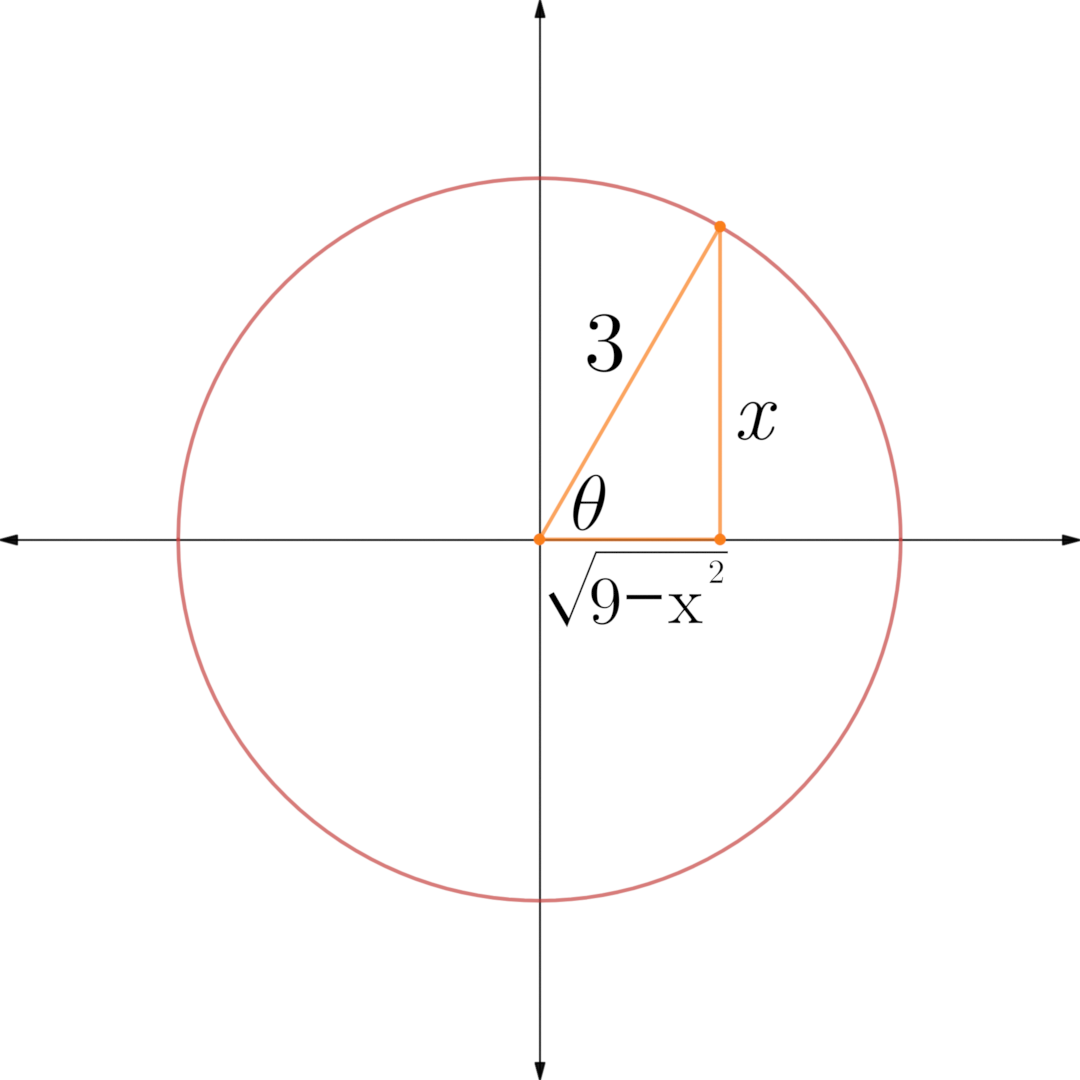
\includegraphics[width=0.35\textwidth]{Blender/Class1Var-NestedTrig-f_0001.png}
    \caption{\label{fig:1}Nested trigonometric functions.}
\end{wrapfigure}

From Figure \ref{fig:1}, simplify the nested trigonometric functions. Use the facts that $\sin\left(\arcsin\left(\frac{x}{3}\right)\right)=\sin\theta$ and $\cos\left(\arcsin\left(\frac{x}{3}\right)\right)=\cos\theta$.
\begin{equation*}
    y=\frac{9\arcsin\left(\frac{x}{3}\right)+9\times\frac{x}{3}\times\frac{\sqrt{9-x^2}}{3}}{2}
\end{equation*}
Simplify and add the constant of integration to yield the following, final integrated equation (equation 6).
\begin{align*}
    y &= \frac{9\arcsin\left(\frac{x}{3}\right)+9\times\frac{x\sqrt{9-x^2}}{9}}{2}\\
    &= \frac{9\arcsin\left(\frac{x}{3}\right)+x\sqrt{9-x^2}}{2}+C\tag{6}
\end{align*}
\newpage
\paragraph{Summary} In this section, the cosecant function and the circle function were integrated. Both have deceptively simple expressions for the amount of work required, yet, after having explored them, it should be clear why each and every step is necessary. Some functions, like the cosecant, require guesswork with only the slightest logical foundation. Others, like the circle function, have a process where every step is intertwined and all shoot for the same goal. Every choice is very careful. In the next section, the functions are in such a state that no amount of algebraic manipulation will make them easier, and some calculus techniques must be used for simplification.
\newpage

\subsubsection{Advanced Calculus Techniques}
\paragraph{Introduction} While a great many functions can be integrated directly or after some algebraic manipulation, there are still more functions that no amount of algebraic work will turn into an integrable form. These functions require specialized calculus rules in order to rewrite them to a simpler form. These techniques will be justified, and then a variety of their implementations will be explored.
\ex This example is concerned with integrating the following function.$$y=\frac{2}{3+5x}$$This process should bring into focus some techniques that have been flirted with in previous examples, such as defining variables as functions and functions in terms of variables. Formally, this process is known as integration by substitution, and it is the purpose of this example to explore this technique in more depth.\par
Let's begin integrating. Write the integrable equation as follows.
\begin{equation*}
    y=\int \frac{2}{3+5x}\, dx
\end{equation*}
Define function, $u$, as $u=3+5x$. Substitute.
\begin{equation*}
    y=\int \frac{2}{u}\, dx
\end{equation*}
Recall from Example 4 the rather dual nature of functions and variables. Even though $u$ is a defined function, it is still possible to integrate with respect to it. Unfortunately, the variable of integration is still $x$. Somehow, there must be a way to define $dx$ in terms of $du$. Luckily, a relation can between $du$ and $dx$ can be found by differentiating $u$ (as a function) with respect to $x$, as follows.
\begin{align*}
    u &= 3+5x\\
    \frac{d}{dx}(u) &= \frac{d}{dx}(3+5x)\\
    \frac{du}{dx} &= \frac{d}{dx}(3)+\frac{d}{dx}(5x)\\
    &= 0+5\\
    &= 5\\
    du &= 5\, dx\\
    dx &= \frac{du}{5}
\end{align*}
Substitute the final line above into where we left off with the integrable equation.
\begin{equation*}
    y=\int \frac{2}{u}\times \frac{du}{5}
\end{equation*}
Multiply fractions; factor out the constant.
\begin{equation*}
    y=\frac{2}{5}\int \frac{du}{u}
\end{equation*}
Employ the rule of integration from Example 2.
\begin{equation*}
    y=\frac{2}{5}\ln|u|
\end{equation*}
Return the substitution and add the constant of integration to yield the following, final integrated equation (equation 7).
\setcounter{equation}{6}
\begin{equation}
    y=\frac{2}{5}\ln|3+5x|+C
\end{equation}
\ex This example is concerned with integrating the following function.$$y=\frac{1}{4+x^2}$$
The first thought of many might be to define a function, $u$, as $u=4+x^2$ and integrate with respect to $u$, but differentiating $u$ to find $dx$ in terms of constants and $du$ fails because$$\frac{du}{dx}=2x$$so a substitiution would still contain the variable, $x$, and we would have a multivariable equation that cannot be evaluated. Therefore, an alternate solution is necessary.\par
Let's begin integrating. Write the integrable equation as follows.
\begin{equation*}
    y=\int \frac{1}{4+x^2}\, dx
\end{equation*}
Define $x$ as $x=2\tan(u)$. The logic will soon become apparent for reasons similar to the integration of the circle equation in Example 4. Substitute.
\begin{equation*}
    y=\int \frac{1}{4+(2\tan(u))^2}\, dx
\end{equation*}
Simplify.
\begin{equation*}
    y=\int \frac{1}{4+4\tan^2(u)}\, dx
\end{equation*}
We also need to define $dx$ in terms of $du$. To do this, differentiate this definition of $x$ with respect to $u$. This can be easily done with the derivative rules in Table \ref{tab:1}, but a short proof follows for clarity.
\begin{align*}
    x &= 2\tan(u)\\
    \frac{d}{du}(x) &= \frac{d}{du}(2\tan(u))\\
    \frac{dx}{du} &= 2\times\frac{d}{dx}\left(\frac{\sin(u)}{\cos(u)}\right)\\
    &= 2\times\left(\frac{\cos(u)\times\cos(u)-\sin(u)\times -\sin(u)}{\cos^2(u)}\right)\\
    &= 2\times\left(\frac{\cos^2(u)+\sin^2(u)}{\cos^2(u)}\right)\\
    &= 2\times\left(\frac{1}{\cos^2(u)}\right)\\
    &= 2\sec^2(u)\\
    dx &= 2\sec^2(u)\, du
\end{align*}
Substitute the final line above into where we left off with the integrable equation.
\begin{equation*}
    y=\int \frac{1}{4+4\tan^2(u)}\times 2\sec^2(u)\, du
\end{equation*}
Multiply fractions; factor out the constant.
\begin{equation*}
    y=\frac{1}{2}\int \frac{\sec^2(u)}{1+\tan^2(u)}\, du
\end{equation*}
Employ the trigonometric identity that $\tan^2(x)+1=\sec^2(x)$ (note that this can be derivied by dividing the Pythagorean trigonometric identity --- $\sin^2(x)+\cos^2(x)=1$ --- by $\cos^2(x)$).
\begin{equation*}
    y=\frac{1}{2}\int \frac{\sec^2(u)}{\sec^2(u)}\, du
\end{equation*}
Simplify.
\begin{equation*}
    y=\frac{1}{2}\int 1\, du
\end{equation*}
Employ the antipower rule.
\begin{equation*}
    y=\frac{1}{2}u
\end{equation*}
Find $u$ in terms of $x$, as follows.
\begin{align*}
    x &= 2\tan(u)\\
    \frac{x}{2} &= \tan(u)\\
    \arctan\left(\frac{x}{2}\right) &= u
\end{align*}
Substitute the final line above into where we left off with the integrable equation and add the constant of integration to yield the following, final integrated equation (equation 8).
\begin{equation}
    y=\frac{1}{2}\arctan\left(\frac{x}{2}\right)
\end{equation}
\ex This example is concerned with integrating the following function.$$y=x\cos(x)$$
This is another equation that may seem deceptively simple. $x$ and $\cos(x)$ are both fairly straightforward to integrate and have their own, respective rules of integration. However, when multiplied, the process becomes more difficult. In the same way the product rule of derivatives is significantly more complicated than the sum and difference rule of derivatives, integration by parts (what can be used to integrate the product of functions) is more complicated than the sum and difference rule of integrals.\par
Let's begin by deriving this rule. This is fairly straightforward from the definiton of the product rule, but a short proof follows, regardless ($u$ and $v$ will stand in for two both differentiable and integrable functions).
\begin{align*}
    \frac{d}{dx}(uv) &= \frac{d}{dx}(u)\times v+u\times\frac{d}{dx}(v)\\
    d(uv) &= du\times v+u\times dv\\
    \int d(uv) &= \int (v\, du+u\, dv)\\
    uv &= \int v\, du + \int u\, dv\\
    uv-\int v\, du &= \int u\, dv\\
    \int u\, dv &= uv-\int v\, du\tag{9}
\end{align*}
Equation 9 above is the final integration by parts formula. However, it may not be immediately obvious how to apply such a formula. As you will recall, $u$ and $v$ are "dummy" functions, that can be set equal to whatever necessary to answer the problem. Likewise, and this is key, $du$ and $dv$ are \emph{related} dummy functions. To elaborate, $du=u'\, dx$ and $dv=v'\, dx$ where $u'$ and $v'$ are the derivatives of $u$ and $v$. Now it may be coming into focus. If we set one function equal to $u$, and the other function times $x$ equal $dv$, we can solve for $du$ and $v$ and rewrite the integrated equation. It may just be that $\int v\, du$ is an easier integral to evaluate, allowing the final antiderivative to be found.\par
Let's begin integrating. Write the integrable equation as follows.
\begin{equation*}
    y=\int x\cos(x)\, dx
\end{equation*}
Define $u$ as $u=x$ and $dv$ as $dv=\cos(x)\, dx$. In this case, $du=1\, dx=dx$ and $v=\sin(x)$ by derivative and integral rules. Rewrite the integrable equation as the right side of equation 9.
\begin{equation*}
    y=x\sin(x)-\int \sin(x)\, dx
\end{equation*}
Evaluate the integral.
\begin{equation*}
    y=x\sin(x)-[-\cos(x)]
\end{equation*}
Simplify and add the constant of integration to yield the following, final integrated equation (equation 10).
\stepcounter{equation}
\begin{equation}
    y=x\sin(x)+\cos(x)+C
\end{equation}
\ex This example is concerned with integrating the following function.$$y=\ln(x)$$
This is certainly a simple function, yet the method of integrating it is not immediately clear. Certainly it cannot be simplified much. There's not a clear expression to be substituted. It is, in fact, integration by parts that is necessary in this case.\par
Let's begin integrating. Write the integrable equation as follows.
\begin{equation*}
    y=\int \ln(x)\, dx
\end{equation*}
To use integration by parts requires the product of two functions, but it appears as if there is only one function present --- $\ln(x)$. However, by the identity property, every function/variable/etc. is equal to itself times 1. Generally, this is not shown, but we will show it now.
\begin{equation*}
    y=\int \ln(x)\times 1\, dx
\end{equation*}
Define $u$ as $u=\ln(x)$ and $dv$ as $dv=1\, dx$. In this case, $du=\tfrac{1}{x}\, dx$ and $v=x$ by derivative and integral rules. Rewrite the integrable equation as the right side of equation 9.
\begin{equation*}
    y= \ln(x)\times x-\int x\times \frac{1}{x}\, dx
\end{equation*}
Simplify.
\begin{equation*}
    y= x\ln(x)-\int 1\, dx
\end{equation*}
Evaluate the integral.
\begin{equation*}
    y= x\ln(x)-[x]
\end{equation*}
Simplify and add the constant of integration to yield the following, final integrated equation (equation 11).
\begin{equation}
    y= x\ln(x)-x+C
\end{equation}
\ex This example is concerned with integrating the following function.$$y=\text{e}^x\cos(x)$$
This clearly necessitates integration by parts as it is the product of two functions. However, integration by parts relies on one function (typically the one being differentiated) getting simpler for the second integral. For example, in Example 7, the derivative of $x$ is 1, so the second integral was just needed trigonometric rules of integration.\par
In this case, $\text{e}^x$ is its own derivative and never changes, while $\cos(x)$ will cycle through positive and negative variations of itself and $\sin(x)$. Therefore, rewrites will not reveal anything \emph{directly} fruitful, and will eventually simplify to the original integrable equation. However, an additional strategy will become apparent after the process starts so we will begin by integrating as we would any function to be integrated by parts.\par
Let's begin integrating. Write the integrable equation as follows.
\begin{equation*}
    y=\int \text{e}^x\cos(x)\, dx
\end{equation*}
It does not particularly matter what we define as $u$ and what we define as $dv$, so let's arbitrarily define $u$ as $u=\text{e}^x$ and $dv$ as $dv=\cos(x)\, dx$. In this case, $du=\text{e}^x\, dx$ and $v=\sin(x)$ by derivative and integral rules. Rewrite the integrable equation as the right side of equation 9.
\begin{equation*}
    y=\text{e}^x\sin(x)-\int \sin(x)\text{e}^x\, dx
\end{equation*}
It appears as if we've accomplished nothing, but in fact, we are on the right track. $\int \sin(x)\text{e}^x\, dx$ is no easier than $\int \text{e}^x\cos(x)\, dx$, but that does not matter. Let's run integration by parts again. This time, however, we cannot choose arbitratily because the if we chose the opposite from the following way, the equation would directly simplify back to where we started. Define $u$ as $u=\text{e}^x$ and $dv$ as $dv=\sin(x)\, dx$. In this case, $du=\text{e}^x\, dx$ and $v=-\cos(x)$. Rewrite the integral in the above equation as the right side of equation 9 (in parenthesees to deal with the subtraction).
\begin{equation*}
    y=\text{e}^x\sin(x)-\left(\text{e}^x(-\cos(x))-\int -\cos(x)\text{e}^x\, dx\right)
\end{equation*}
Simplify.
\begin{align*}
    y &= \text{e}^x\sin(x)-\left(-\text{e}^x\cos(x)+\int \cos(x)\text{e}^x\, dx\right)\\
    &= \text{e}^x\sin(x)+\text{e}^x\cos(x)-\int \text{e}^x\cos(x)\, dx\\
\end{align*}
It may seem as if we're back where we started with $\int \text{e}^x\cos(x)\, dx$, but, in reality, we now have two other terms that will not cancel first. These two facts (that we have the original integral and that we have other terms) are key. Recall that $y$ does not just equal what it does directly above, but everything else since the original integrable equation as well. This means that we can set any two (or three or all) of the above equations equal to each other. In this case, set the original equation equal to the last one.
\begin{equation*}
    \int \text{e}^x\cos(x)\, dx = \text{e}^x\sin(x)+\text{e}^x\cos(x)-\int \text{e}^x\cos(x)\, dx
\end{equation*}
This is it --- \emph{combine like terms}.
\begin{equation*}
    2\int \text{e}^x\cos(x)\, dx = \text{e}^x\sin(x)+\text{e}^x\cos(x)
\end{equation*}
Divide both sides by 2.
\begin{equation*}
    \int \text{e}^x\cos(x)\, dx = \frac{\text{e}^x\sin(x)+\text{e}^x\cos(x)}{2}
\end{equation*}
Return the substitution of the original integrable equation and add the constant of integration to yield the following, final integrated equation (equation 12).
\begin{equation}
    y = \frac{\text{e}^x\sin(x)+\text{e}^x\cos(x)}{2}+C
\end{equation}
\paragraph{Summary} In this section, a great deal of, again, relatively simple-looking functions were integrated. Some, such as the natural log function, were nothing but a special function and its argument, similar to cosecant in Section 1.1.2, but took ingeniously simple observations to integrate. Others, such as $\text{e}^x\cos(x)$ required persistence and a loose conceptualizaiton of like terms. However, as has been the theme throughout Section 1.1, each initial integrable equation could be simplified to a more workable form where previously mentioned rules could be applied. Furthermore, each equation only had one variable with which to deal and $y$ was left mostly alone except for Example 9. These patterns will not continue, however, as we move onto Section 1.2.
\newpage


\subsection{Functions of \emph{x} and \emph{y} (Differential Equations)}
\subsubsection{Simple}
\paragraph{Introduction} In this section, we will explore several functions of $x$ and $y$ that can be integrated through relatively straightforward means, once the mental block surrounding two variables is passed. Furthermore, a method of examining such functions and predicting their integral will be explored.
\ex This example is concerned with integrating the following function.$$\frac{dy}{dx}=\frac{-x}{y}$$
The most notable difference between this function and all others so far is that it is of two variables, $x$ and $y$. Secondly, because of this, its derivative can no longer be shown as a function defined implicitly in $y$, but must be formally shown as $\tfrac{dy}{dx}$. This means that, since this equation cannot be solved for $y$ without integration, this differential equation$^[$\footnote{An equation with at least one $\frac{dy}{dx}$ term of some degree as a component.}$^]$ does not describe a line that is present at some points in the coordinate plane and not others, but \emph{slopes} at each and every combination of $x$ and $y$. This is often shown as a slope field, such as the two shown below in Figure \ref{fig:2}.

\begin{figure}[h!]
    \centering
    \begin{subfigure}[b]{0.4\linewidth}
        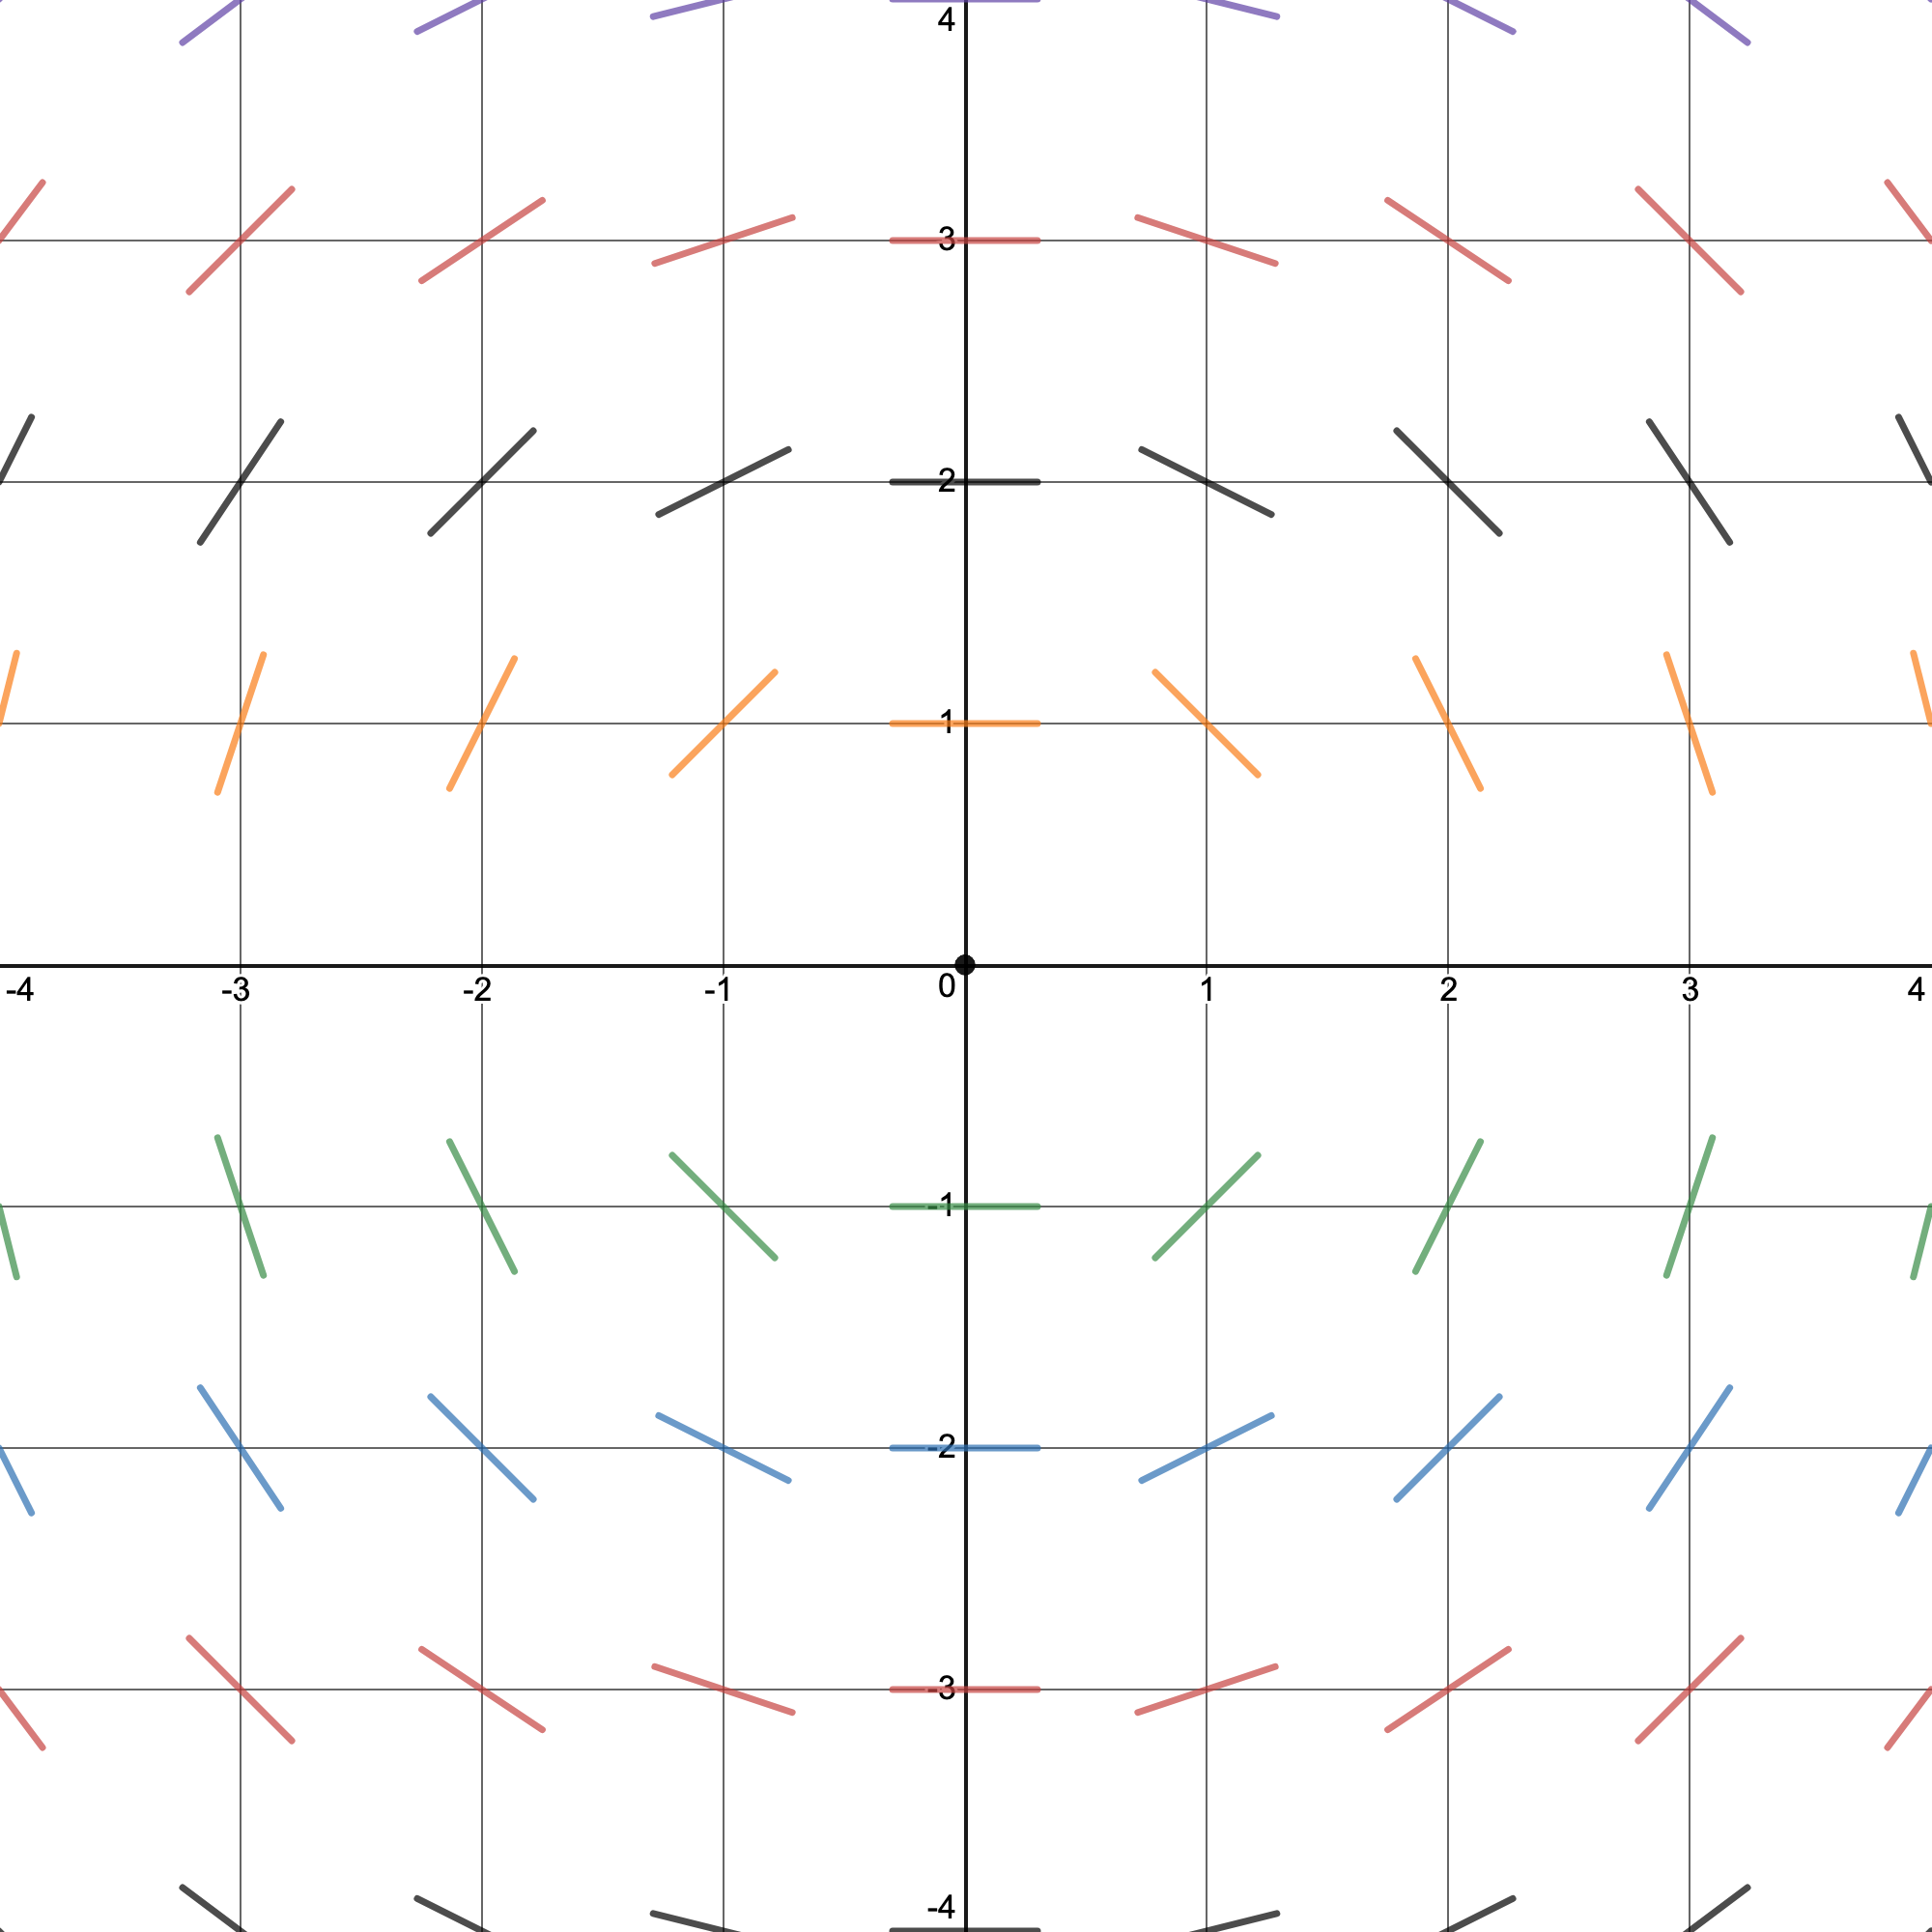
\includegraphics[width=\linewidth]{Blender/SlopeField-10a.png}
        \caption{Slope field for $\tfrac{-x}{y}$.}
        \label{fig:2a}
    \end{subfigure}\hspace{3em}
    \begin{subfigure}[b]{0.4\linewidth}
        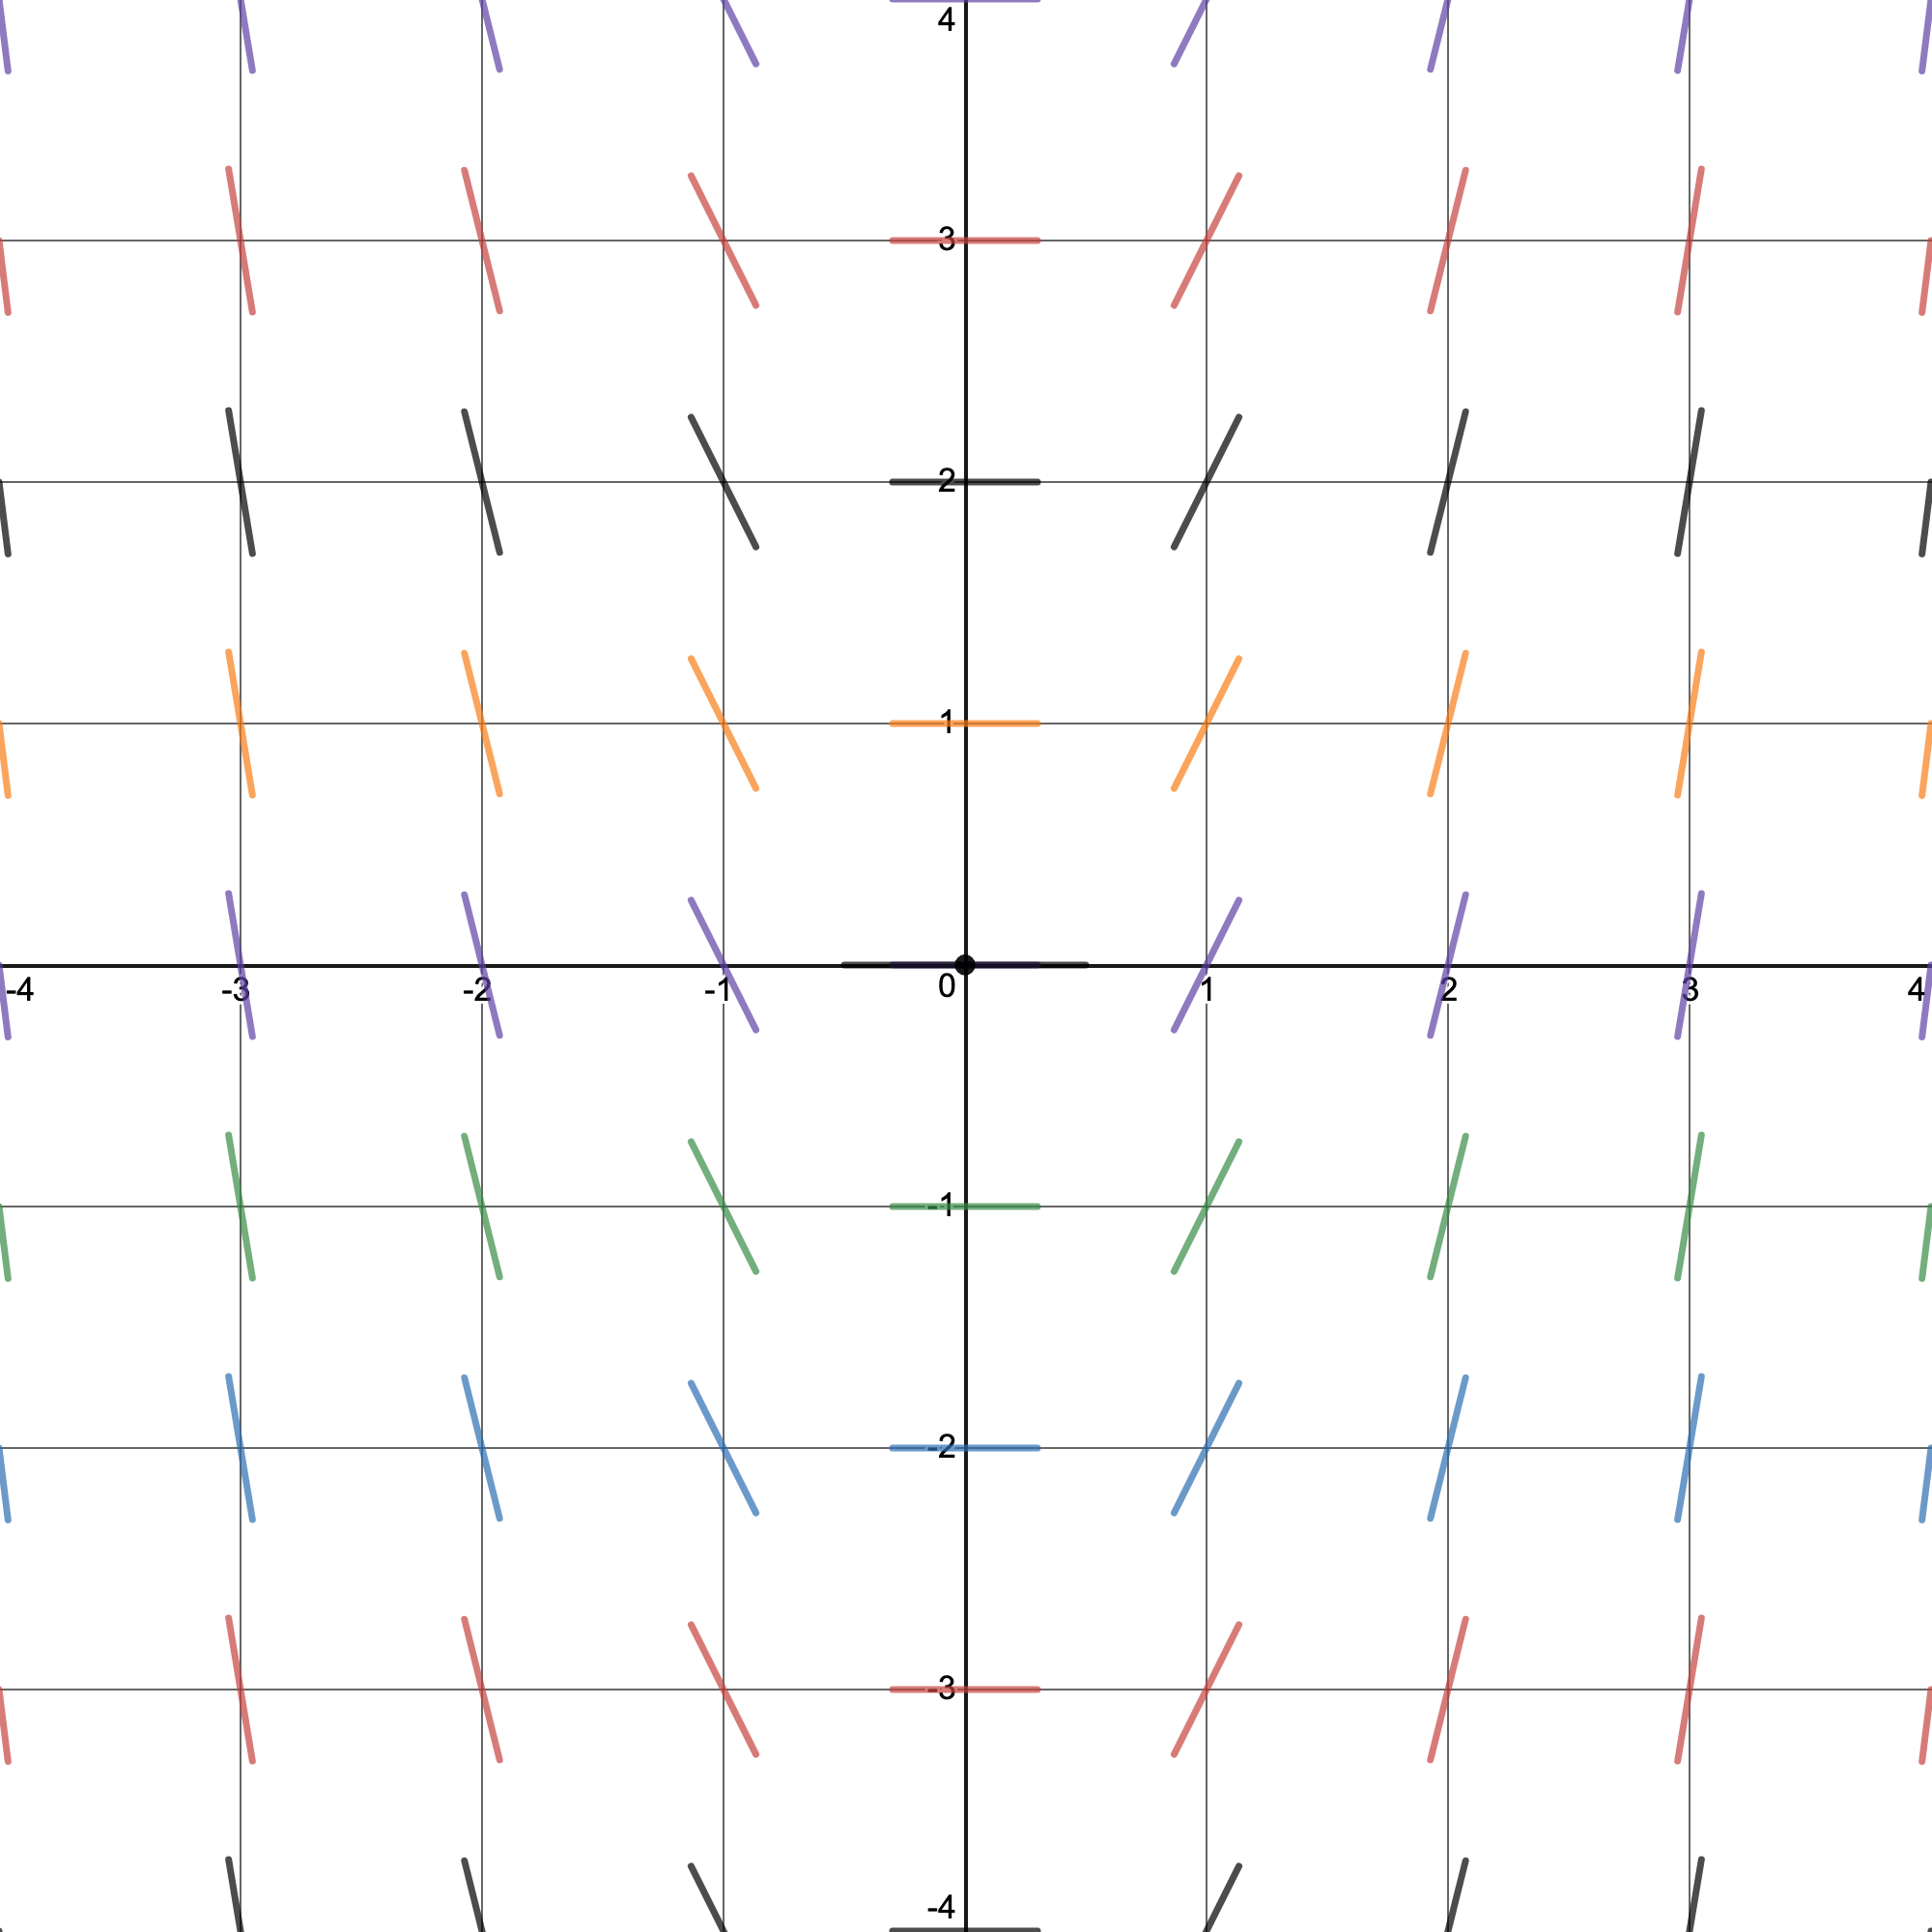
\includegraphics[width=\linewidth]{Blender/SlopeField-10b.png}
        \caption{Slope field for $2x$.}
        \label{fig:2b}
    \end{subfigure}
    \caption{Two slope fields.}
    \label{fig:2}
\end{figure}

The slope field shown in Figure \ref{fig:2a} shows the differential equation given in this example on one unit intervals, while the slope field in Figure \ref{fig:2b} shows the derivative of the parabola, $x^2$. What is done to generate each is that at every point to be shown, the $x$ and $y$ (if necessary) coordinates are plugged into the differential equation and a short line segment with this slope is placed at that point. For example, at point,\ (1,1) in Figure \ref{fig:2a}, we can find the slope to be $\tfrac{-1}{1}=-1$. If we look at (1,1) in Figure \ref{fig:2a}, we can see that the line segment does appear to have a slope of $-1$.\par
Slope fields can also give an estimate of what the shape may look like and what its constant of integration may do to it as it varies. For example, in Figure \ref{fig:2b}, which we know is the slope field for the parabola, $x^2$, we can sort of make out a series of parabolas stacked vertically. This tells us that if we solve the differential equation,$$\frac{dy}{dx}=2x$$we can expect to find an equation for a parabola and the constant of integration will make it vary vertically. Likewise, when looking at Figure \ref{fig:2a}, we can expect to find an equation for a circle that grows and shrinks radially in size as $C$ varies. Clearly, slope fields are a good way to take a peak at where we're going.\par
Let's begin integrating. Write the integrable equation as follows.
\begin{equation*}
    \frac{dy}{dx}=\frac{-x}{y}
\end{equation*}
This clearly differs from the initial integrable equations in every other example so far. Whereas the others had a variable ($y$) defined in terms of an integral symbol, an integrand, and a variable of integration, this is still just the initial differential equation. However, as was mentioned before, every function that an example first introduced could have been written after $\tfrac{dy}{dx}$ (one could then multiply both sides by $dx$ and integrate both sides to get what was called the initial integrable equation, but these steps were skipped for simplicity's sake).\par
Regardless, what's important now is to isolate the variables and their respective differentials on either side of the equals sign. Cross multiply to achieve this.
\begin{equation*}
    y\, dy=-x\, dx
\end{equation*}
Take the integral of both sides. This is allowed for the same reason that you can add, subtract, multiply, or divide both sides by the same thing --- as long as the integrals have the same (or related) bounds, you can integrate both sides.
\begin{equation*}
    \int y\, dy=\int -x\, dx
\end{equation*}
Employ the antipower rule twice.
\begin{equation*}
    \frac{y^2}{2}=\frac{-x^2}{2}
\end{equation*}
Add the constants of integration. It is important that the constant(s) of integration is/are added immediately after integrating for reasons that will be more fully explored in Example 12. For now, it will suffice to say that as the equation is solved for $y$, operations performed on the various terms must also be performed on the constant of integration.
\begin{equation*}
    \frac{y^2}{2}+C=\frac{-x^2}{2}+C
\end{equation*}
Since a constant ($C\in \mathbb{R}$) plus or minus a constant ($C\in \mathbb{R}$) is just a constant ($C\in \mathbb{R}$), we can eliminate one of the two constants of integration.
\begin{equation*}
    \frac{y^2}{2}=\frac{-x^2}{2}+C
\end{equation*}
Multiply both sides by 2.
\begin{equation*}
    y^2=-x^2+2C
\end{equation*}
Two times a constant ($C\in \mathbb{R}$) is a constant ($C\in \mathbb{R}$).
\begin{equation*}
    y^2=-x^2+C
\end{equation*}
Move the variables to the same side to yield the following, final integrated equation (equation 13).
\begin{equation}
    x^2+y^2=C
\end{equation}
Though we could solve this equation for $y$, it should be clear at this point that this is, indeed, the equation for a circle. Since $C$ is where $r^2$ would be in a regular circle equation, we can understand that $C$ controls not the vertical position of the circle, but its radial size, just as the slope field in Figure \ref{fig:2a} predicted.
\ex This example is concerned with integrating the following function.$$\frac{dy}{dx}=\frac{-2x-y}{x+2y}$$
Though this may initially look far harder than the equation discussed in Example 10, it is actually the same level of difficulty with one additional step covered by an aforementioned technique. In other words, while all functions heretofore explored have required differing techniques (or have built on previously used techniques) this is an example of a radically different looking funcition that I would classify in the same category as the one in Example 10.\par
Let's begin integrating. Write the integrable equation as follows.
\begin{equation*}
    \frac{dy}{dx}=\frac{-2x-y}{x+2y}
\end{equation*}
Cross multiply.
\begin{equation*}
    (x+2y)\, dy=(-2x-y)\, dx
\end{equation*}
Take the integral of both sides.
\begin{equation*}
    \int (x+2y)\, dy=\int (-2x-y)\, dx
\end{equation*}
Employ the sum and difference rule twice. Note that we could also have chosen to skip the above step and distributed the differentials to the terms in parenthesees before taking integrals of both terms at the same time. In other words, one can justify the sum and difference rule by noting that one can think of the integral symbol and differential as variables that are multiplied by the integrand and can be distributed or factored at will.
\begin{equation*}
    \int x\, dy+\int 2y\, dy=\int -2x\, dx-\int y\, dx
\end{equation*}
Manipulate the equation to isolate the terms whose variable is the same as its corresponding differential and those whose variable is different than its corresponding differential on different sides of the equals sign.
\begin{equation*}
    \int 2y\, dy-\int -2x\, dx=-\int y\, dx-\int x\, dy
\end{equation*}
Employ the antipower rule twice on the terms on the left side of the equals sign; rewrite the right side (factor out the negative, switch terms).
\vspace{-1em}
\begin{equation*}
    \frac{2y^2}{2}-\frac{-2x^2}{2}=-\left(\int x\, dy+\int y\, dx\right)
\end{equation*}
Simplify the left side.
\vspace{-1em}
\begin{equation*}
    y^2+x^2=-\left(\int x\, dy+\int y\, dx\right)
\end{equation*}
On the right side, the observant reader may notice that $x\, dy+y\, dx$ is nothing but an expansion of the product rule, and integrating should yield $xy$. However, this will be proved, instead, using integration by parts. Rewrite the left term on the right side of the equals sign as the right side of equation 9.
\begin{equation*}
    y^2+x^2=-\left(xy-\int y\, dx+\int y\, dx\right)
\end{equation*}
Simplify and add the constant of integration to yield the following, final integrated equation (equation 14).
\begin{align*}
    y^2+x^2 &= -\left(xy\right)\\
    y^2+x^2+xy &= 0\\
    x^2+xy+y^2 &= C\tag{14}
\end{align*}
\vspace{-2em}
\ex This example is concerned with integrating the following function.$$\frac{dy}{dx}=3y$$
This may seem familliar to the reader at first glance --- it describes the rate of density-dependent growth with a $k$ value of 3. Furthermore, evaluating this differential equation is arguably even more simple than some past examples, but the real implications of this example lie in its treatment of the constant of integration. While both Examples 10 and 11 led to variations of conic sections, this function is best solved for $y$ after integration and will allow us to explore different purposes of $C$ more clearly, as was mentioned in Example 10.\par
Let's begin integrating. Write the integrable equation as follows.
\begin{equation*}
    \frac{dy}{dx}=3y
\end{equation*}
Multiply both sides by $dx$; divide both sides by $y$.
\begin{equation*}
    \frac{dy}{y}=3\, dx
\end{equation*}
Take the integral of both sides.
\begin{equation*}
    \int \frac{dy}{y}=\int 3\, dx
\end{equation*}
Employ the rule of integration from Example 2 and the antipower rule.
\begin{equation*}
    \ln|y|=3x
\end{equation*}
Add the constant of integration.
\begin{equation*}
    \ln|y|=3x+C
\end{equation*}
By the converse of the definition of the logarithm, if $\log_a(c)=b$, then $a^b=c$. Employ this definition to rewrite the above equation.
\begin{equation*}
    |y|=\text{e}^{3x+C}
\end{equation*}
Rewrite with a plus or minus sign to eliminate the absolute value symbol.
\begin{equation*}
    y=\pm\text{e}^{3x+C}
\end{equation*}
Employ the rule of exponents that $a^{m+n}=a^ma^n$.
\begin{equation*}
    y=\pm\text{e}^{3x}\text{e}^C
\end{equation*}
Reorder the terms.
\begin{equation*}
    y=\pm\text{e}^C\text{e}^{3x}
\end{equation*}

\begin{figure}[h!]
    \centering
    \begin{subfigure}[b]{0.4\linewidth}
        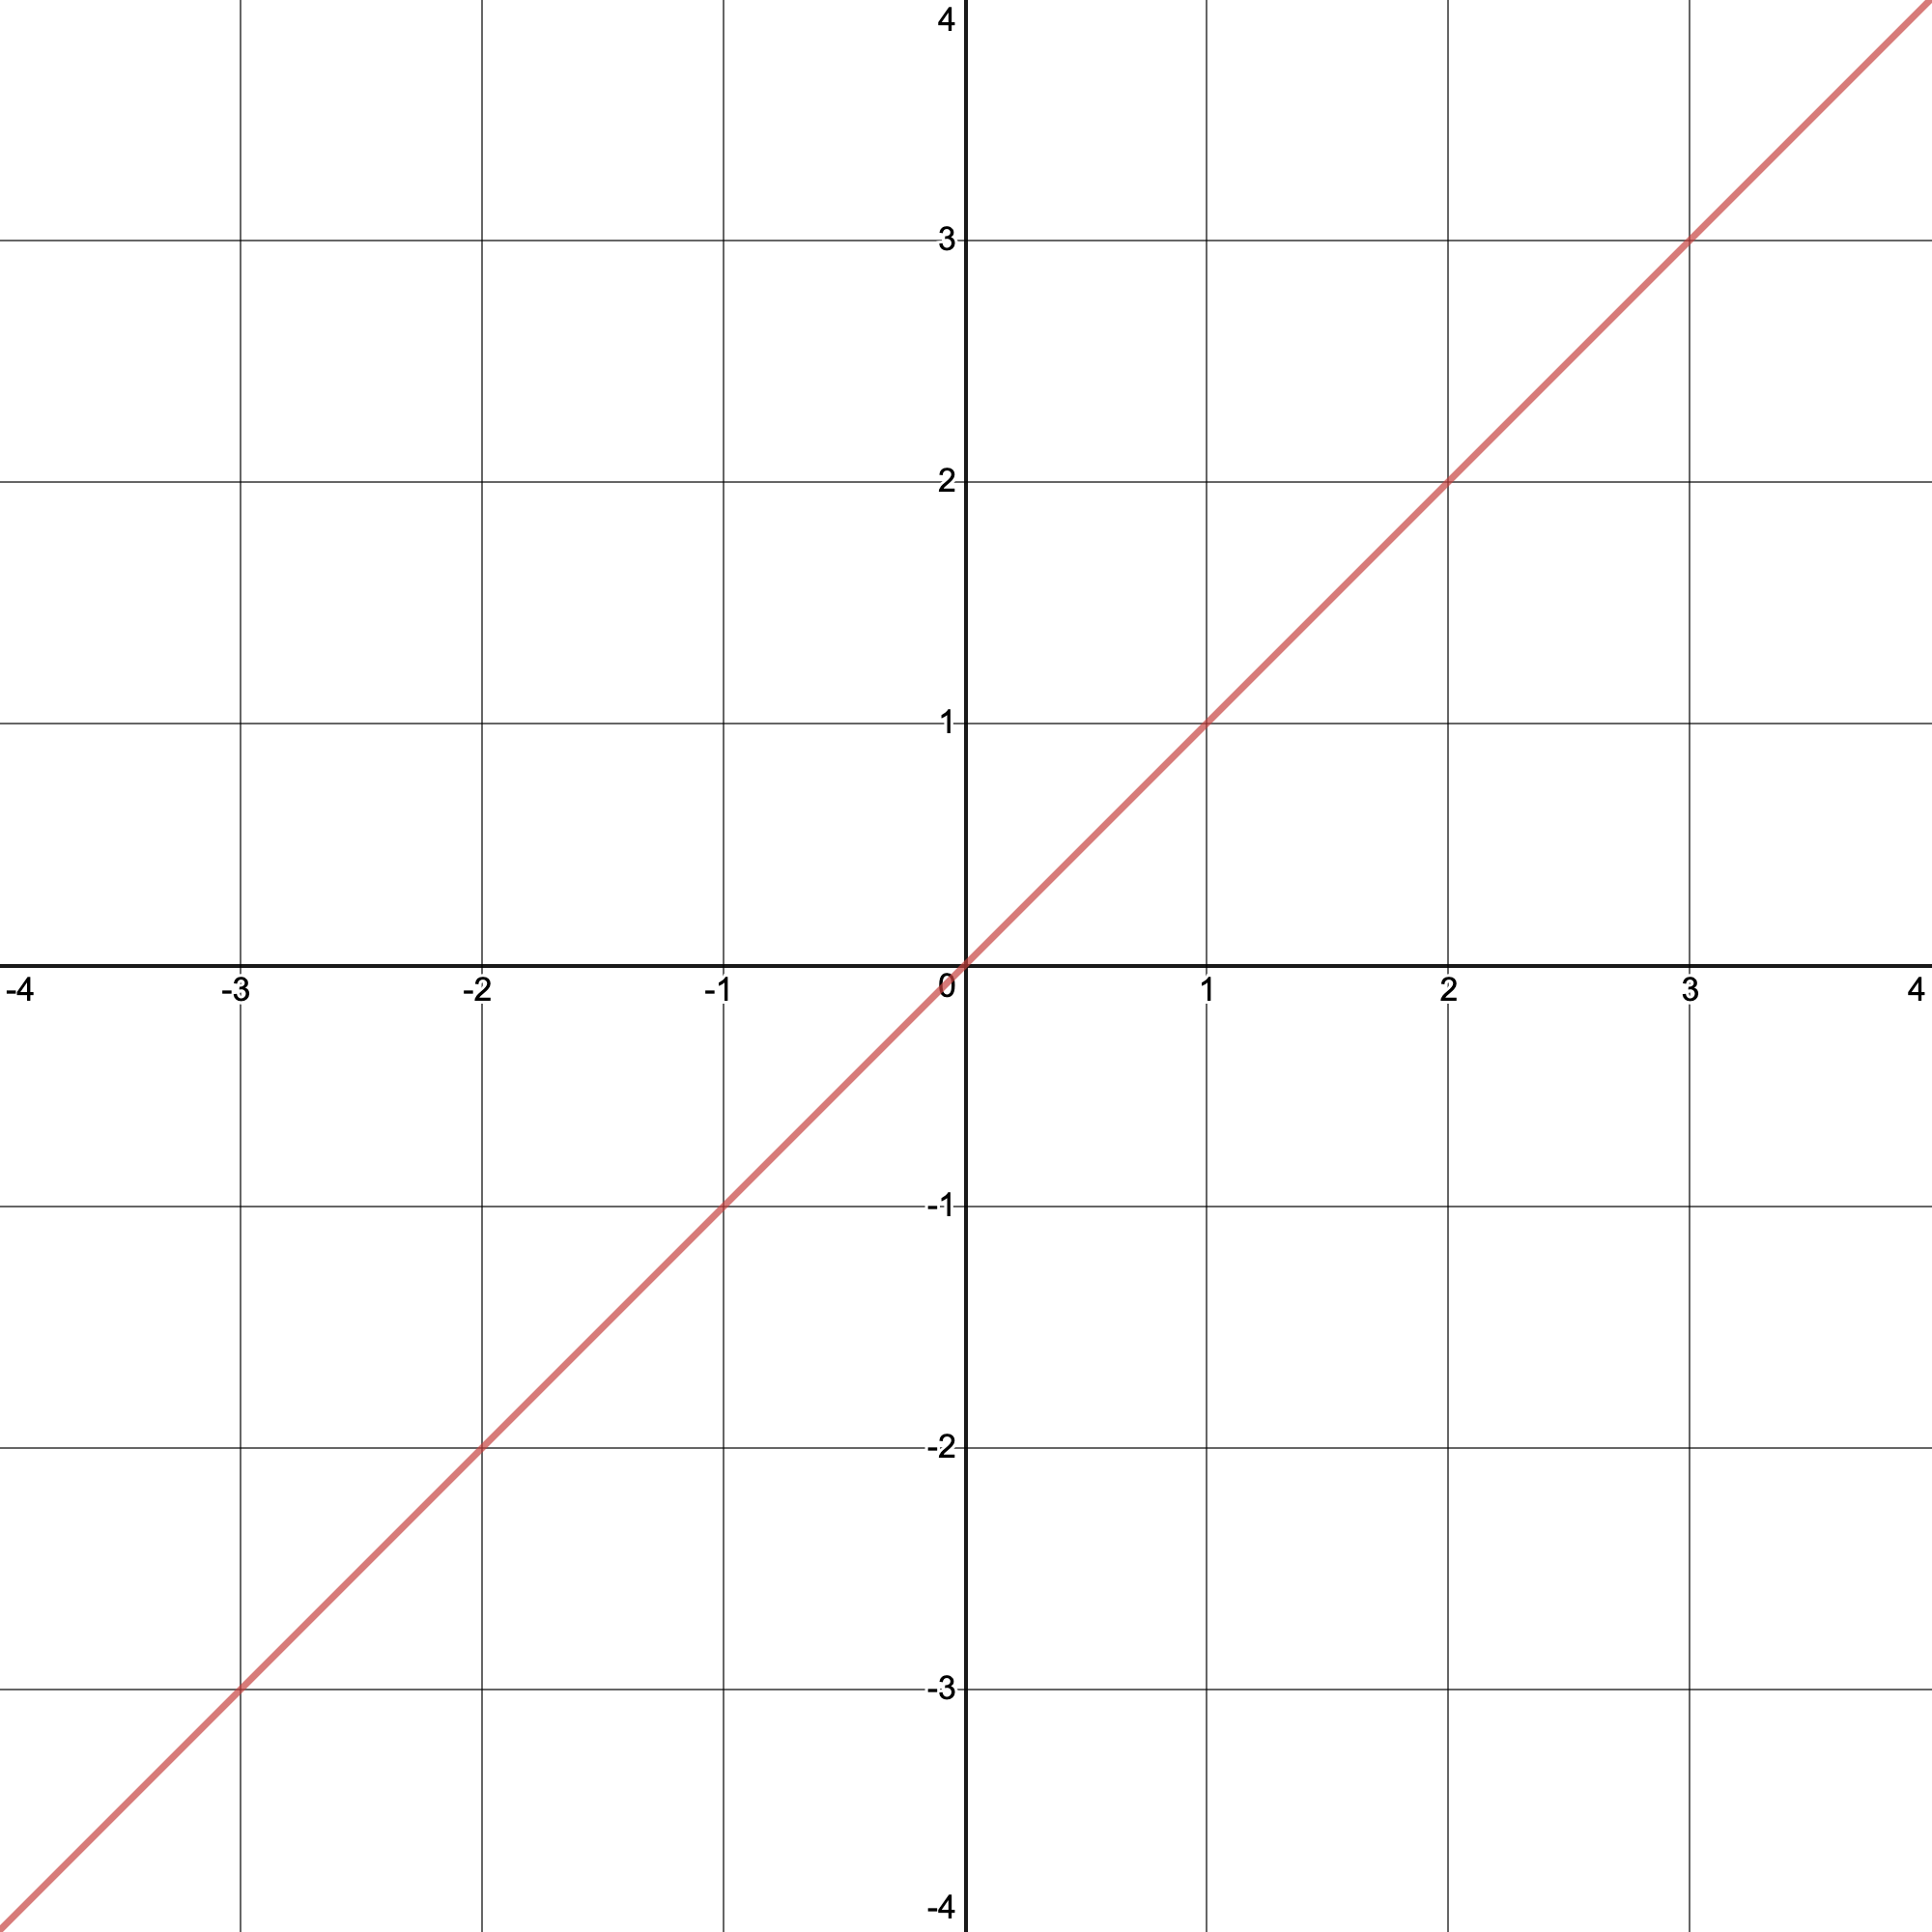
\includegraphics[width=\linewidth]{Blender/C-straight.png}
        \caption{Variation across $\mathbb{R}$.}
        \label{fig:3a}
    \end{subfigure}\hspace{3em}
    \begin{subfigure}[b]{0.4\linewidth}
        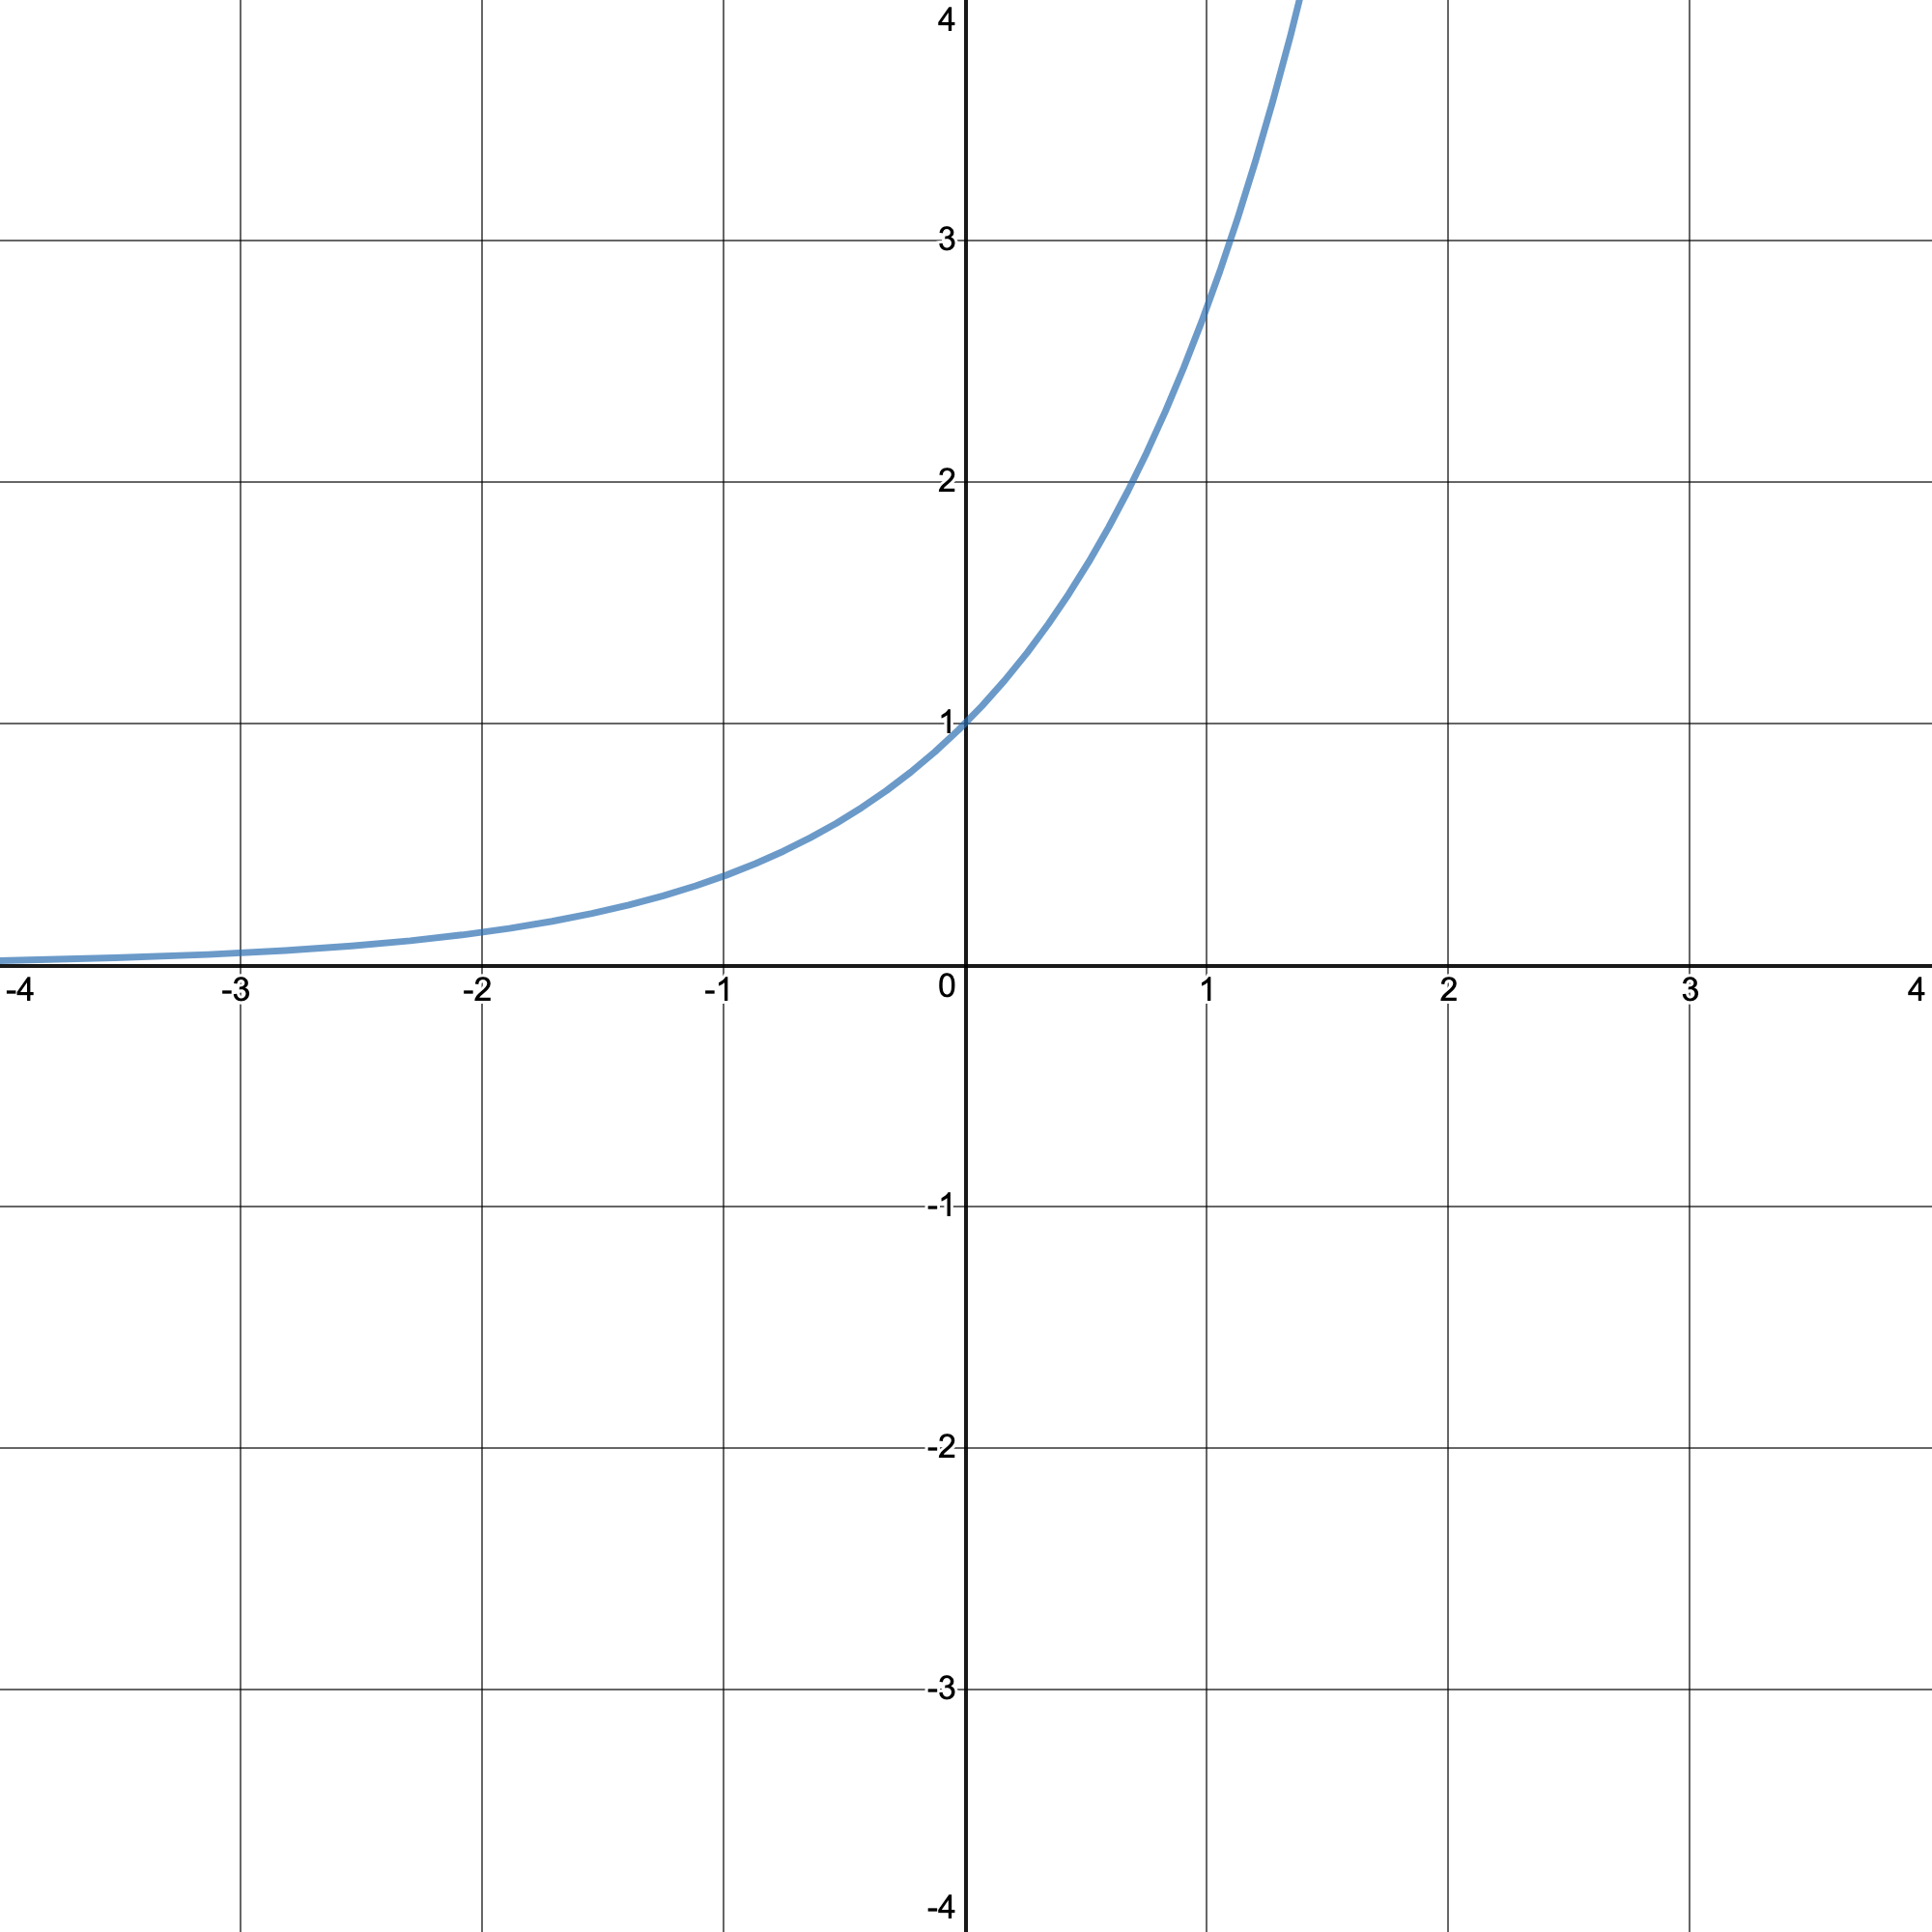
\includegraphics[width=\linewidth]{Blender/C-e^x.png}
        \caption{Variation across $\mathbb{R}_{>0}$.}
        \label{fig:3b}
    \end{subfigure}
    \caption{Different ways $C$ can vary.}
    \label{fig:3}
\end{figure}

At this point, it should be clear why it is necessary to add in the constant of integration immediately after integrating. Whereas the manipulations in the last two equations did not vary the range of the constant of integration ($C\in\mathbb{R}$), these manipulations have. $\text{e}^C$ does not have a range among the real numbers, but a range among the positive real numbers (excluding zero), as $C$ varies. This is because of the graphical interpretation of $C$, as seen in Figure \ref{fig:3}. Whereas $C$ varying among the real numbers can be visualised as a straight line (where every real number \emph{is} within its range), as in Figure \ref{fig:3a}, $\text{e}^C$ varies only in the positive numbers as $C$ varies among the real numbers, as in Figure \ref{fig:3b}. That being said, the plus or minus sign means that $C$ really varies among all of the real numbers except zero. This type of constant is expressed as $A$, where $A$ is directly defined as $A=\pm\text{e}^C$ and has a range $A\in(-\infty,0)\cup(0,\infty)$.\par
Rewrite the equation with which we left off with $A$ to yield the following, final integrated equation (equation 15).
\stepcounter{equation}
\begin{equation}
    y=A\text{e}^{3x}
\end{equation}
\paragraph{Summary} Throughout this section, several functions of two variables have been integrated. The same techniques that were used in Section 1.1 were employed here, but integration occured on both sides of the equals sign with respect to not just $x$, but $x$ and $y$, independently.\par
Furthermore, the uses of the constant of integration were expanded from simply varying a function horizontally (see Figure \ref{fig:2b}) to radially (see Figure \ref{fig:2a}) and beyond (see Example 12). In Figure \ref{fig:2}, some of these variations were explored graphically through slope fields, and in Figure \ref{fig:3}, direct limits on the bounds of $C$ were discussed.\par
Notably, all of these functions involved terms or groups of terms that were multiplied by each other or divided by each other. When unmitigated addition and subtraction are introduced, things can become more complicated, as seen in Section 1.2.2.
\newpage

\subsubsection{Advanced Algebraic Techniques}
\paragraph{Introduction} In this section, two functions with addition and subtraction are analyzed. One is a monomial that is rather simply processed with a recurring technique. The other is a binomial in $y$ which requires a rather ingenious algebraic technique and some advanced processing after integration to solve for $y$.
\ex This example is concerned with integrating the following function.$$\frac{dy}{dx}=1+y$$
As was mentioned in the summary of Section 1.2.1, this is clearly a function where the main (and arguably sole) component is addition. It looks rather simple, and, indeed, its integration is a good launching point for more broadly exploring addition and subtraction in two-variable functions.\par
Let's begin integrating. Write the integrable equation as follows.
\begin{equation*}
    \frac{dy}{dx}=1+y
\end{equation*}
Multiply both sides by $dx$; divide both sides by $1+y$.
\begin{equation*}
    \frac{dy}{1+y}=dx
\end{equation*}
Take the integral of both sides.
\begin{equation*}
    \int\frac{dy}{1+y}=\int dx
\end{equation*}
Define $u$ as $u=1+y$. In this case, $du=dy$ by derivative rules. Make these two substitutions.
\begin{equation*}
    \int\frac{du}{u}=\int dx
\end{equation*}
Employ the rule of integration from Example 2 and the antipower rule.
\begin{equation*}
    \ln|u|=x
\end{equation*}
Add the constant of integration.
\begin{equation*}
    \ln|u|=x+C
\end{equation*}
Return the substitution.
\begin{equation*}
    \ln|1+y|=x+C
\end{equation*}
Employ the definition of the lorarithm to rewrite the above equation.
\begin{equation*}
    |1+y|=\text{e}^{x+C}
\end{equation*}
Rewrite with a plus or minus sign to eliminate the absolute value symbol.
\begin{equation*}
    1+y=\pm\text{e}^{x+C}
\end{equation*}
Employ the rule of exponents that $a^{m+n}=a^ma^n$.
\begin{equation*}
    1+y=\pm\text{e}^x\text{e}^C
\end{equation*}
Substitute $A$ for $\pm\text{e}^C$.
\begin{equation*}
    1+y=A\text{e}^x
\end{equation*}
Subtract 1 from both sides of the equals sign to yield the following, final integrated equation (equation 16).
\begin{equation}
    y=A\text{e}^x-1
\end{equation}
\ex This example is concerned with integrating the following function.$$\frac{dy}{dx}=y^2+2y-24$$
This function is a progression from both Examples 12 and 13. It is a polynomial in $y$ and will require techniques used in those aforementioned examples as well as a new technique called partial fractions$^[$\footnote{\label{fot:1}A method of splitting a single fraction with two or more elements multiplied in the denominator into the sum or difference of two or more resultant fractions, which subsequently often have lower degree terms in the denominator.}$^]$.\par
Let's begin integrating. Write the integrable equation as follows.
\begin{equation*}
    \frac{dy}{dx}=y^2+2y-24
\end{equation*}
Multiply both sides by $dx$; divide both sides by $y^2+2y-24$.
\begin{equation*}
    \frac{dy}{y^2+2y-24}=dx
\end{equation*}
Take the integral of both sides; separate $dy$ from the fraction on the left side of the equals sign.
\begin{equation}
    \int \frac{1}{y^2+2y-24}\, dy=\int dx
\end{equation}
Now, we run into a roadblock that we avoided in Example 13. The denominator of the $y$ fraction is a second-degree polynomial. This means that if we defined a function, $u$, as $u=y^2+2y-24$, the substitution for $dx$ would be $\frac{du}{2y+2}$ by differentiation rules. This means that $y$ would still be in the integrand, and we would now be trying to integrate a multivariable ($y$ and $u$) function with only one variable of integration --- an impossible task. Therefore, we need a different technique, i.e. partial fractions.\par
According to the definition of the method of partial fractions in Footnote \ref{fot:1}, it may be possible to separate this large fraction into two with first-degree denominators, which could be separated with the sum or difference rule of integrals. The following will guide the reader through this method.\par
Isolate the fraction for consideration --- we'll return to the integrable equation later. To begin, factor the denominator. One could solve it algebraically with the quadratic formula, but the keen eye will discern that two factors of -24 are -4 and 6, which sum to 2 (the $b$ coefficient). Therefore, rewrite the denominator with these factors in mind.
\begin{equation*}
    \frac{1}{(y-4)(y+6)}
\end{equation*}
Set this fraction equal to the sum of two fractions, as shown below.
\begin{equation}
    \frac{1}{(y-4)(y+6)}=\frac{A}{y-4}+\frac{B}{y+6}
\end{equation}
$A$ and $B$ are variable numerators. What this statement claims is that there are two fractions, with denominators $y-4$ and $y+6$ that, with some as-of-yet undiscovered numerators, sum to the original fraction. Now, the logical basis of partial fractions may be coming into focus. When fractions are added, the first step is to find a common denominator. Though an LCD (least common denominator) can be beneficial, one surefire way to find a common denominator is by multiplying the two denominators under question. However, to modify the denominator also requires modifying the numerator, i.e. multiplying each fraction by a clever form of one.\par
Multiply each fraction on the right side of the equals sign by the other fraction's denominator divided by that same denominator.
\begin{equation*}
    \frac{1}{(y-4)(y+6)}=\frac{A}{y-4}\times\frac{y+6}{y+6}+\frac{B}{y+6}\times\frac{y-4}{y-4}
\end{equation*}
Simplify.
\begin{equation*}
    \frac{1}{(y-4)(y+6)}=\frac{A(y+6)}{(y-4)(y+6)}+\frac{B(y-4)}{(y+6)(y-4)}
\end{equation*}
Now, the fractions on the right side have the same denominator, so they can be added (add the numberators over the common denominator).
\begin{equation*}
    \frac{1}{(y-4)(y+6)}=\frac{A(y+6)+B(y-4)}{(y-4)(y+6)}
\end{equation*}
Multiply both sides by $(y-4)(y+6)$.
\begin{equation*}
    1=A(y+6)+B(y-4)
\end{equation*}
Distribute. Add $0y$, or zero (this will not disturb equality), to the left side of the equation.
\begin{equation*}
    0y+1=yA+6A+yB-4B)
\end{equation*}
Now, we have one equation and two unknown variables...or so it seems. In fact, we actually can write a system of two equations from this one equation. Since the only operators are addition and subtraction, the first-degree terms (those with a $y$) and the zeroeth-degree terms (those without a $y$) must respectively sum to zero and one because of their equality with the left side of the equation. In other words, $Ay+By=0y$ and $6A-4B=1$. By dividing out the $y$ on both sides of the first equation and pairing it with the second, we get the following system of equations.
\begin{align*}
    A+B &= 0\\
    6A-4B &= 1
\end{align*}
Solve this system as follows.
\begin{equation*}
    A=-B
\end{equation*}
\begin{align*}
    6(-B)-4B &= 1\\
    -10B &= 1\\
    B &= -\frac{1}{10}\tag{19}
\end{align*}
\begin{align*}
    A + -\frac{1}{10} &= 0\\
    A &= \frac{1}{10}\tag{20}
\end{align*}
Substitute equations 19 and 20 into equation 18.
\begin{equation*}
    \frac{1}{(y-4)(y+6)}=\frac{\frac{1}{10}}{y-4}+\frac{-\frac{1}{10}}{y+6}
\end{equation*}
Simplify the right side.
\begin{align*}
    \frac{1}{(y-4)(y+6)} &= \frac{1}{10(y-4)}+\frac{-1}{10(y+6)}\\
    &= \frac{1}{10y-40}-\frac{1}{10y+60}\tag{21}
\end{align*}
Substitute the right side of equation 21 into equation 17.
\begin{equation*}
    \int \left(\frac{1}{10y-40}-\frac{1}{10y+60}\right)\, dy=\int dx
\end{equation*}
Employ the sum and difference rule.
\begin{equation*}
    \int \frac{1}{10y-40}\, dy-\int \frac{1}{10y+60}\, dy=\int dx
\end{equation*}
Define $u$ as $u=10y-40$ and $v$ as $v=10y+60$. In the first case, $dy=\frac{du}{10}$, while in the second case, $dy=\frac{dv}{10}$. Substitute four times.
\begin{equation*}
    \int \frac{1}{u}\times \frac{du}{10}-\int \frac{1}{v}\times \frac{dv}{10}=\int dx
\end{equation*}
Multiply fractions; factor out the constants.
\begin{equation*}
    \frac{1}{10}\int \frac{du}{u}-\frac{1}{10}\int \frac{dv}{v}=\int dx
\end{equation*}
Employ the rule of integration from Example 2 twice and the antipower rule once.
\begin{equation*}
    \frac{1}{10}\ln|u|-\frac{1}{10}\ln|v|=x
\end{equation*}
Add the constant of integration.
\begin{equation*}
    \frac{1}{10}\ln|u|-\frac{1}{10}\ln|v|=x+C
\end{equation*}
Return the substitutions.
\begin{equation*}
    \frac{1}{10}\ln|10y-40|-\frac{1}{10}\ln|10y+60|=x+C
\end{equation*}
At this point, we have successfully integrated the initial differential equation. However, we will go a few steps farther and solve for $y$, as we have in the previous few examples. Some steps, especially with regard to manipulating $C$ will be combined for the sake of space and since they have been described in great detail in past examples.\par
Anyway, multiply both sides by 10.
\begin{equation*}
    \ln|10y-40|-\ln|10y+60|=10x+C
\end{equation*}
Employ the property of logarithms that $\log_a(b)-\log_a(c)=\log_a\left(\frac{b}{c}\right)$.
\begin{equation*}
    \ln\abs{\frac{10y-40}{10y+60}}=10x+C
\end{equation*}
Employ the definition of the logarithm to rewrite the above equation.
\begin{equation*}
    \abs{\frac{10y-40}{10y+60}}=\text{e}^{10x+C}
\end{equation*}
Manipulate by steps from previous examples.
\begin{equation*}
    \frac{10y-40}{10y+60}=A\text{e}^{10x}
\end{equation*}
Multiply both sides by $10y+60$.
\begin{equation*}
    10y-40=A\text{e}^{10x}(10y+60)
\end{equation*}
Distribute.
\begin{equation*}
    10y-40=10Ay\text{e}^{10x}+60A\text{e}^{10x}
\end{equation*}
Combine all terms with a $y$ on the left side of the equals sign and all terms without a $y$ on the right side of the equals sign.
\begin{equation*}
    10y-10Ay\text{e}^{10x}=60A\text{e}^{10x}+40
\end{equation*}
Factor out a $y$ from each term on the left side of the equation.
\begin{equation*}
    y\left(10-10A\text{e}^{10x}\right)=60A\text{e}^{10x}+40
\end{equation*}
Divide both sides by $\left(10-10A\text{e}^{10x}\right)$.
\begin{equation*}
    y=\frac{60A\text{e}^{10x}+40}{10-10A\text{e}^{10x}}
\end{equation*}
Divide both the numerator and denominator of the fraction by 10 to yield the following, final integrated equation (equation 22).
\setcounter{equation}{21}
\begin{equation}
    y=\frac{6A\text{e}^{10x}+4}{1-A\text{e}^{10x}}
\end{equation}
\paragraph{Summary} As was referenced in the introduction, addition in monomials can be handled through integration by substitution after combining similar variables on the same side of the equals sign. A polynomial is definitely more complicated. The one that was analyzed in Example 14 above required the complex process of partial fractions followed by a series of algebraic manipulations that culminated in a rather messy fraction --- a far cry from some of the other, more clean results in this paper.\par
In the next section, only one function will be integrated, but the trick requires a thorough mastery of techniques of integration \emph{and} differentiation to spot.
\newpage

\subsubsection{Advanced Calculus Techniques}
\paragraph{Introduction} In this section, only one function will be analyzed. It has addition and subtraction, like the functions in Section 1.2.2, but requires radically different calculus-based techniques to rewrite it into an integrable form. Unlike Example 14, the answer is almost as simple as the differential equation, but still has its own little gems (explored in the Summary).\par
This function requires the reader to draw deep on calculus knowledge and intimately consider differentiation as well as integration for the first time in this paper. Lastly, it is still not technically a multivariable function, but it does require techniques that, perhaps, most closely resemble a multivariable function of any explored herein.
\ex This example is concerned with integrating the following function.$$\frac{dy}{dx}=x+y$$
As was previously alluded to, this is the most complex function that we will be algebraically integrating. It appears extremely simple --- just the addition of the two variables, yet the trick here requires the product rule, of all things, a specialized function, and some rather ingenious algebraic and calculus manipulation. However, the final answer is not nearly as complicated as the one in Example 14.\par
Let's begin integrating. Write the integrable equation as follows.
\begin{equation*}
    \frac{dy}{dx}=x+y
\end{equation*}
The first step is not necessarily obvious. If we multiply both sides by $dx$ and employed the sum and difference rule, one integral would work out via the antipower rule. However, the other would require integrating $y$ with respect to $x$, an impossible task. Effectively, it does not appear as if there is a way to pair each variable with its differential, so an alternate method is required.\par
Let's get $y$ and its derivative ($\frac{dy}{dx}$ or $y'$) on the same side of the equation. Subtract $y$ from both sides.
\begin{equation*}
    \frac{dy}{dx}-y=x
\end{equation*}
We cannot integrate yet, but we are getting closer. Think back to differentiation. When else does the addition or subtraction of a variable and its derivative come up in calculus? Though it has not been directly dealt with in this paper, Example 11 did reference the product rule when trying to evaluate $\int x\, dy + \int y\, dx$. As a review, the product rule is the antithesis to integration by parts, and can be stated in any of the following ways$^[$\footnote{The prime (apostrophe) of a function designates its derivative.}$^]$, where $u$ and $v$ are differentiable functions.
\begin{align*}
    \frac{d}{dx}(uv) &= \frac{d}{dx}(u)\times v+u\times \frac{d}{dx}(v)\\
    &= \frac{du}{dx}\times v+u\times \frac{dv}{dx}\tag{23}\\
    &= u'v+uv'
\end{align*}
What appeals about the product rule is that if we can transform the left side of where we left off with the integrable equation into a format that directly resembles the right side of equation 23, then we can eliminate the addition by rewriting as the left side of equation 23. The right side of equation 23 is close to our situation above, but not a perfect match. We have a variable and its derivative separated by an addition/subtraction operator, but we do not have the second variable/derivative pair. The closest we can get right now to transforming the left side of where we left off into product-rule format is by showing the $1$ and $-1$ as "functions" multiplied by $y$ and its derivative, as follows.
\begin{equation*}
    1\times\frac{dy}{dx}+-1\times y=x
\end{equation*}
Unfortunately, $1$ and $-1$ do not share a derivative/integral calculus relation, so we cannot simply compress the left side above into the left side of the definition of the product rule. However, we can multiply both sides of the equation by a function, $u$, that can resolve this issue.\par
Multiply both sides by $u$, an as-of-yet undefined function.
\stepcounter{equation}
\begin{equation}
    u\times\frac{dy}{dx}+-u\times y=ux
\end{equation}
Now we're getting somewhere. The leftmost term, $uy'$, is practically directly related to the product rule. However, $-uy$ does not equal $u'y$, but it needs to, so set these terms equal to each other$^[$\footnote{This is the key and it cannot be undersold. In trying to establish a link between equation 23 and the integrable equation, we need an exact parallel, or equality. By setting the two terms that need to be equal equal to each other, we can solve for a function, $u$, except we use calculus to solve for a function instead of algebra to solve for a variable.}$^]$.
\begin{equation*}
    -uy=u'y
\end{equation*}
Divide both sides by $y$.
\begin{equation*}
    -u=u'
\end{equation*}
Rewrite $u'$ in Leibniz's notation.
\begin{equation*}
    \frac{du}{dx}=-u
\end{equation*}
Now, we have a differential equation which we can solve to find the function, $u$, that we need to suit our needs. Divide both sides by $u$; multiply both sides by $dx$.
\begin{equation*}
    \frac{du}{u}=-dx
\end{equation*}
Take the integral of both sides.
\begin{equation*}
    \int \frac{du}{u}=\int -dx
\end{equation*}
Employ the rule of integration from Example 2.
\begin{equation*}
    \ln|u|=-x
\end{equation*}
Employ the definition of the logarithm to rewrite the above equation.
\begin{equation*}
    |u|=\text{e}^{-x}
\end{equation*}
Rewrite with a plus or minus sign to eliminate the absolute value symbol.
\begin{equation*}
    u=\pm\text{e}^{-x}
\end{equation*}
At this point, it would seem that there are two potential functions that satisfy the conditions for $u$. This is perhaps strange, but nevertheless true. I'll explain: Since $u$ is multiplied through the entirety of equation 24, if $u$ is positive, all terms in equation 24 will be positive. If $u$ is negative, all terms in equation 24 will be negative, but multiplying by $-1$ makes equation 24 equivalent to the first case. In effect, either definition of $u$ \emph{does} satisfy the necessary conditions.\par
Substitute the positive definiton (for simplicity's sake) of $u$ into equation 24.
\begin{equation*}
    \text{e}^{-x}\times\frac{dy}{dx}+-\text{e}^{-x}\times y=\text{e}^{-x}x
\end{equation*}
By the definition of $u$, $-\text{e}^{-x}=\frac{d}{dx}\left(\text{e}^{-x}\right)$, a fact that can be confirmed by derivative or integral rules. As such, substitute $\frac{d}{dx}\left(\text{e}^{-x}\right)$ for $-\text{e}^{-x}$.
\begin{equation*}
    \text{e}^{-x}\times\frac{dy}{dx}+\frac{d}{dx}\left(\text{e}^{-x}\right)\times y=\text{e}^{-x}x
\end{equation*}
At this point, the left side of the above equation directly resembles equation 23 where $u$ (in equation 23) is related to $\text{e}^{-x}$ while $v$ is related to $y$. Therefore, the product rule can be used to rewrite the left side of the above equation, as follows.
\begin{equation*}
    \frac{d}{dx}\left(y\text{e}^{-x}\right)=\text{e}^{-x}x
\end{equation*}
Define $w$ as $w=y\text{e}^{-x}$ and rewrite the equation above. This simplifies the multivariate differential for the integration step. Make this substitution.
\begin{equation*}
    \frac{dw}{dx}=\text{e}^{-x}x
\end{equation*}
Now, it may become obvious how far we've come. As of defining $w$, we have rewritten the addition of two variables as a differential equation equal to the multiplication of two functions of the same variable. Furthermore, there is still a differential of that variable ($dx$) in the equation, so this can be evaluated via integration by parts. When integrated, $dw$ will become $w$, at which point the substitution can be returned and the equation solved for $y$. This process follows.\par
Multiply both sides by $dx$.
\begin{equation*}
    dw=\text{e}^{-x}x\, dx
\end{equation*}
Take the integral of both sides.
\begin{equation*}
    \int dw=\int\text{e}^{-x}x\, dx
\end{equation*}
Define $u$ as $u=x$ and $dv$ as $dv=\text{e}^{-x}\, dx$. In this case, $du=dx$ and $v=-\text{e}^{-x}$ by derivative and integral rules. Rewrite the right side of the above equation as the right side of equation 9.
\begin{equation*}
    \int dw=-x\text{e}^{-x}-\int -\text{e}^{-x}\, dx
\end{equation*}
Employ the antipower rule and the the definitions of function $u$ (that $\frac{du}{dx}=-\text{e}^{-x}$ and $u=\text{e}^{-x}$).
\begin{equation*}
    w=-x\text{e}^{-x}-\text{e}^{-x}
\end{equation*}
Add the constant of integration.
\begin{equation*}
    w=-x\text{e}^{-x}-\text{e}^{-x}+C
\end{equation*}
Return the substitution of $w$.
\begin{equation*}
    y\text{e}^{-x}=-x\text{e}^{-x}-\text{e}^{-x}+C
\end{equation*}
Divide both sides by $\text{e}^{-x}$ to solve for $y$.
\begin{equation*}
    y=-x-1+\frac{1}{\text{e}^{-x}}\times C
\end{equation*}
Employ the rule of exponents that $a^{-m}=\frac{1}{a^m}$.
\begin{equation*}
    y=-x-1+\frac{1}{\frac{1}{\text{e}^{x}}}\times C
\end{equation*}
Multiply the complex fraction by $1=\frac{\text{e}^{x}}{\text{e}^{x}}$ and simplify. Note that this is, indeed, $C$ out front as opposed to $A$.
\begin{equation*}
    y=-x-1+C\text{e}^{x}
\end{equation*}
Reorder the terms to put the term with a positive coefficient in front to yield the following, final integrated equation (equation 25).
\begin{equation}
    y=C\text{e}^{x}-x-1
\end{equation}
\paragraph{Summary} And so ends the integration of the most interesting non-multivariate algebraically integrable function I have come across. Throughout Section 1.2, the reader may have wondered how integrating a two-variable function can still yield a one variable function. Furthermore, he or she may note that, if we take Example 15 for instance, the derivative of the final integrated equation does not appear to be equal to the initial integrable equation. However, it is --- there is simply an extra step after differentiation to return to the initial integrable equation. This will be briefly explored below.\par
Let's differentiate equation 25. Begin with the initial differentiable equation,$$y=C\text{e}^{x}-x-1$$and separate terms with the sum and difference rule and differentiate with rules that have already been explored to yield$$\frac{dy}{dx}=C\text{e}^x-1$$Note that as $C$ is just a constant, it can be factored out during the differentiation process and thus does not change. This may appear to be completely different from $x+y$, but it is actually equivalent. If $x$ is added to both sides of the initial differentiable equation, the equality becomes$$x+y=C\text{e}^x-1$$If the substitution is made, the reader will see the initial integrable equation from Example 15 as it should be.\par
Through this exercise, it may also have become clear why a differential equation in $x$ and $y$ can still be termed a one-variable function. A true \emph{multivariable} function might look like $z=x+y$, but because $\frac{dy}{dx}$ is so inherently related to $y$, $x$, and planar graphing in general, all functions do stay true to the title and can be classified as functions of one-variable.\par
Section 2 will continue to explore one-variable functions, but these will not be able to be integrated by any rules discussed as of yet in this paper.
\newpage



\section{Approximations of Nonintegrable Functions}
\subsection{Restricted Estimates}
\paragraph{Introduction} In this section, the idea of a nonintegrable function will be explained. Once the reader is convinced that such a function exists, two methods of approximating definite integrals will be explored (for the same function so that the accuracy of the two approaches can be compared).
\ex This example is concerned with integrating the following function.$$y=\sin(x^2)$$
As has been referneced above, this function cannot be integrated with any techniques discussed thus far. Every function so far could either be directly integrated using a set of techniques (antipower rule, $\frac{du}{u}$ rule, etc.) or could be manipulated to such a form that these rules then applied.\par
However, sticking with the theme of simple functions that require complex techniques, it is the lack of complication of this function that makes it possible to see why any previous techniques will not work. Let's begin with Example 1. Is this a polynomial function that can be integrated via the sum and difference rule and the antipower rule? No. It's got a binomial, but this part of it is nested within a non-polynomial function. How about Example 2? Is there any way to turn this function into a case of $\frac{du}{u}$? No, there is not. The derivative of this function is $x\cos(x^2)$ which cannot be introduced directly through an algebraic rewrite or through a clever form of one \'a la Example 3, no matter how much Table \ref{tab:1} is analyzed. Example 4 deals with the very specific case of a difference of perfect squares under a radical, so it is not applicable. Example 5 does not work for the same reason as Example 2-3. Example 6 does not work for a similar reason to Example 4. Example 7-9 rely on integration by parts, but $\sin(x^2)$ is only one function. The Example 8 technique of calling $1$ a function also does not work in this case because $2x^2\cos(x^2)$ is no easier to integrate than $\sin(x^2)$ (infact, rewriting this with integration by parts brings the reader right back to $\sin(x^2)$). Obviously, nothing from Example 10-15 will work because these are differential equations and require rewrites so that Example 1-9 techniques can be used.\par

\begin{figure}[h!]
    \centering
    \begin{subfigure}[b]{0.4\linewidth}
        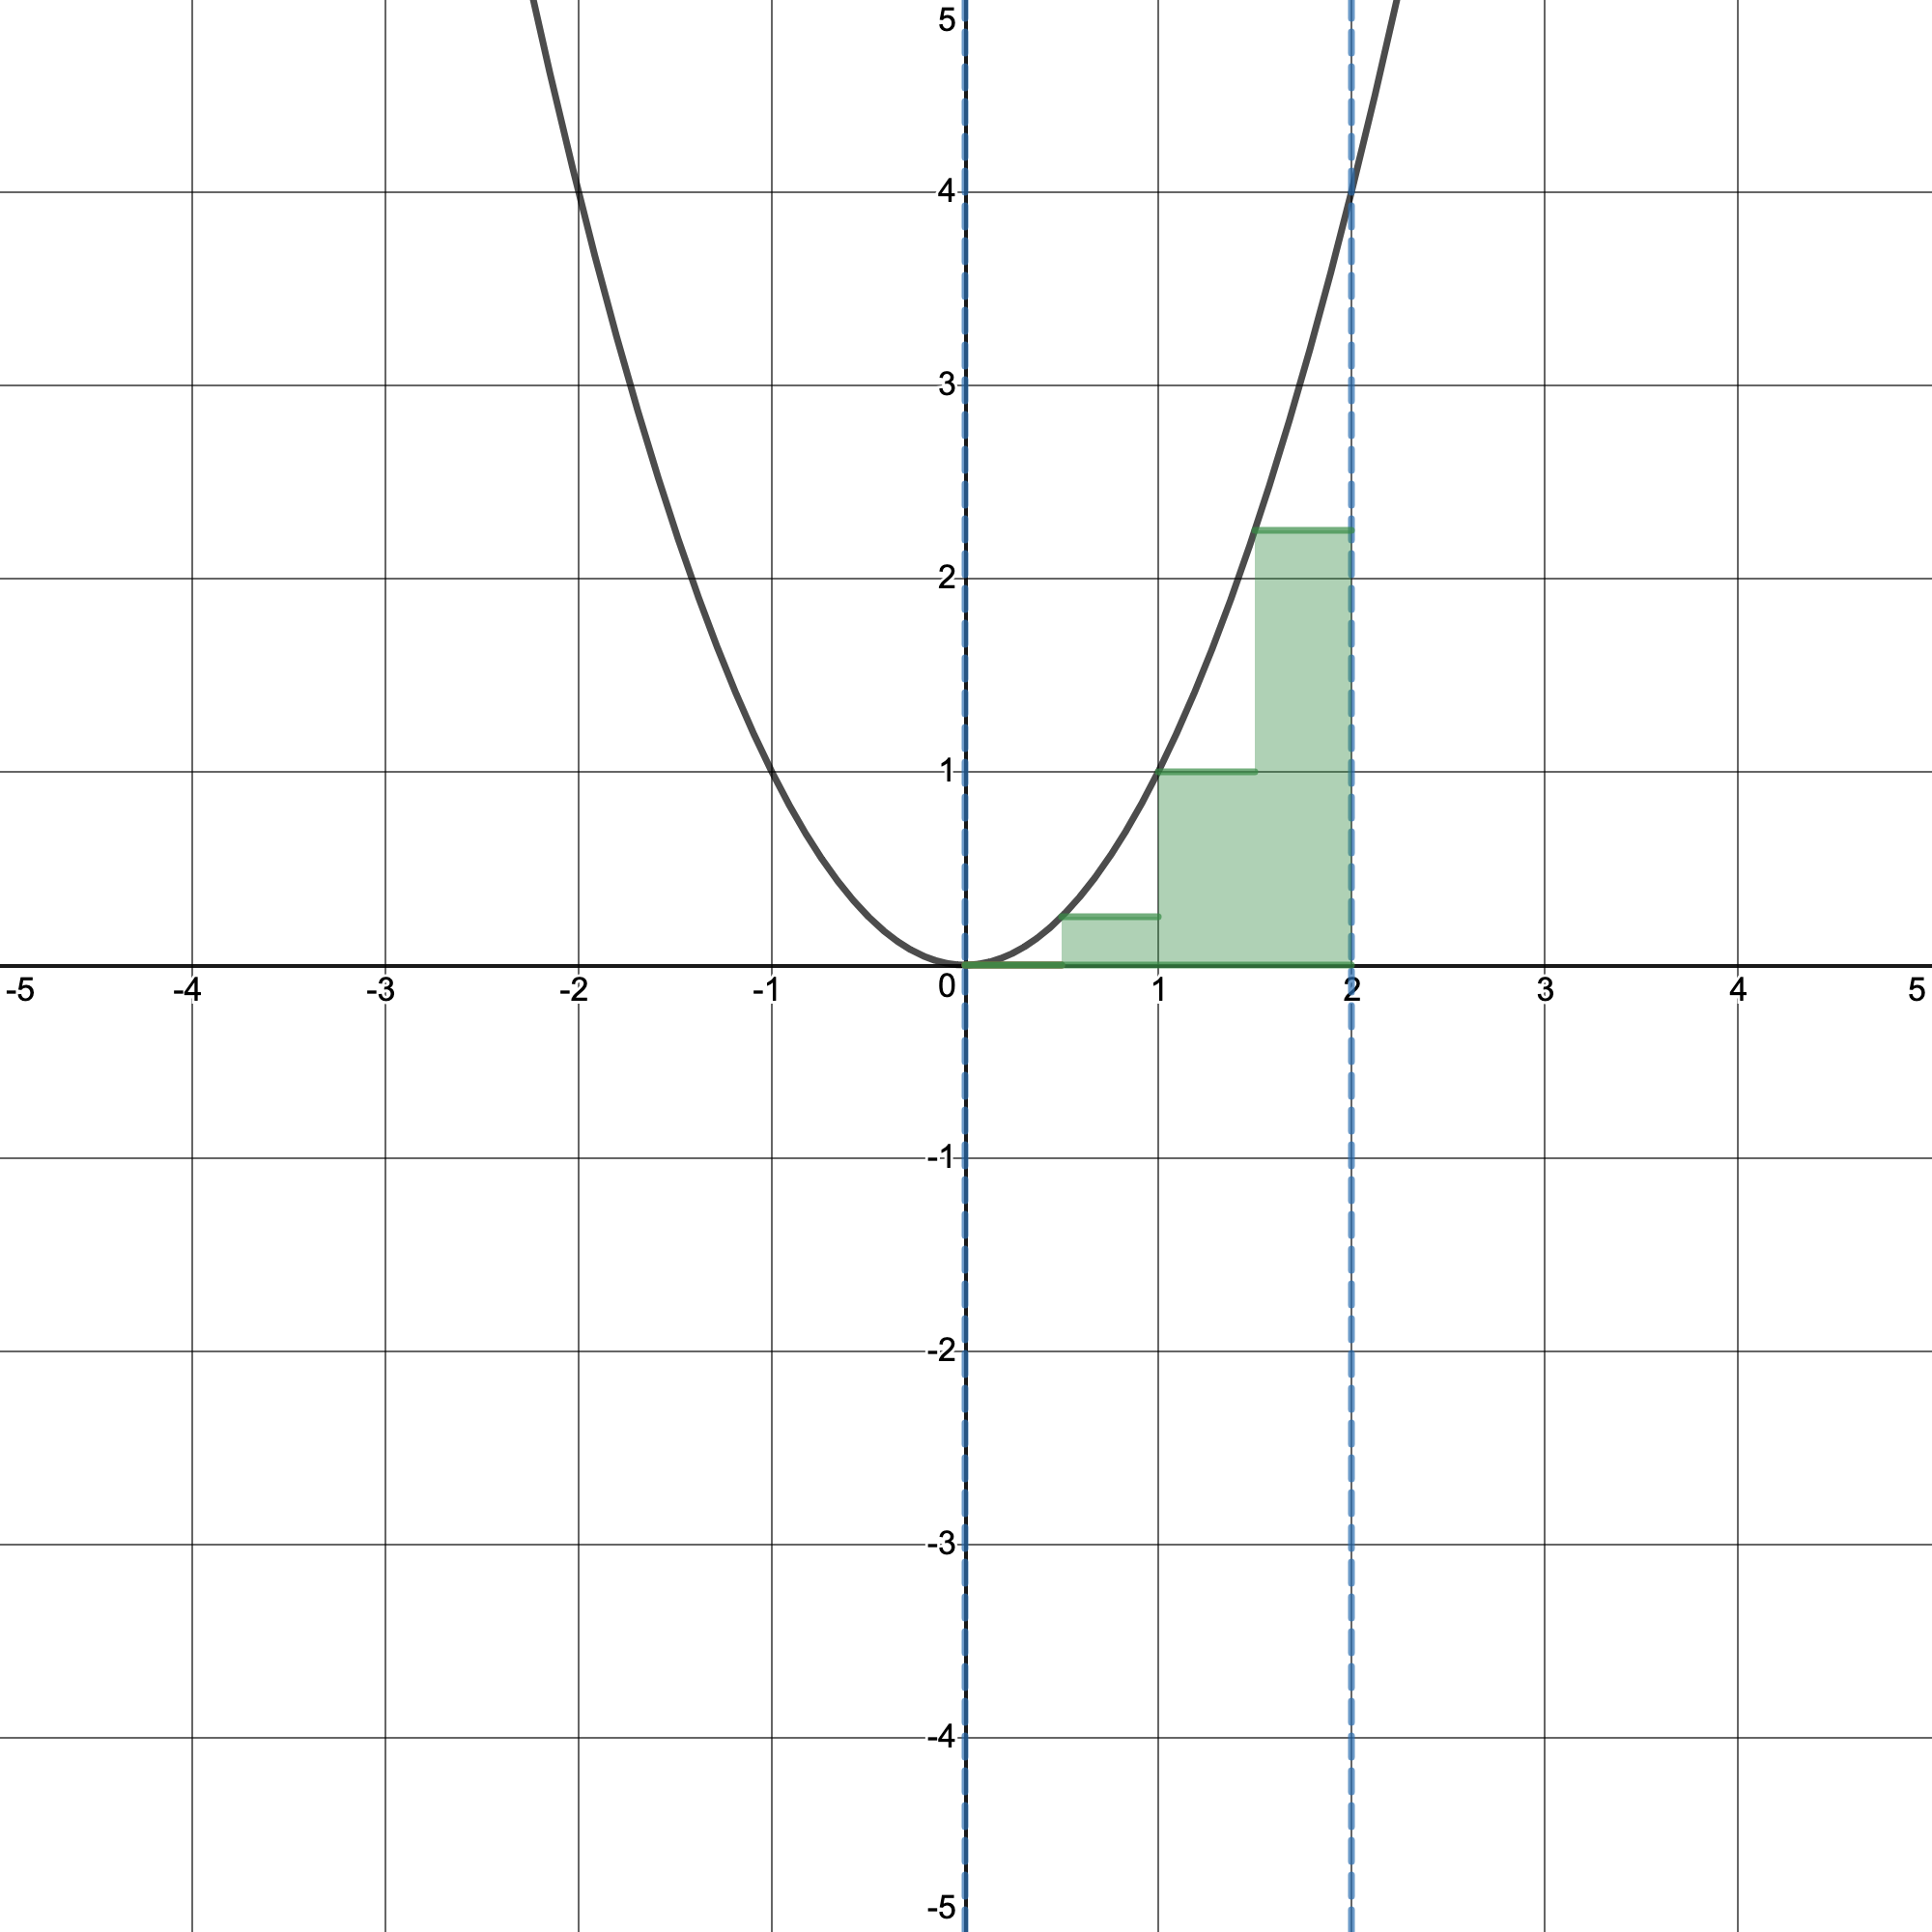
\includegraphics[width=\linewidth]{Blender/Rsum4.png}
        \caption{Four subintervals ($n=4$).}
        \label{fig:4a}
    \end{subfigure}\hspace{3em}
    \begin{subfigure}[b]{0.4\linewidth}
        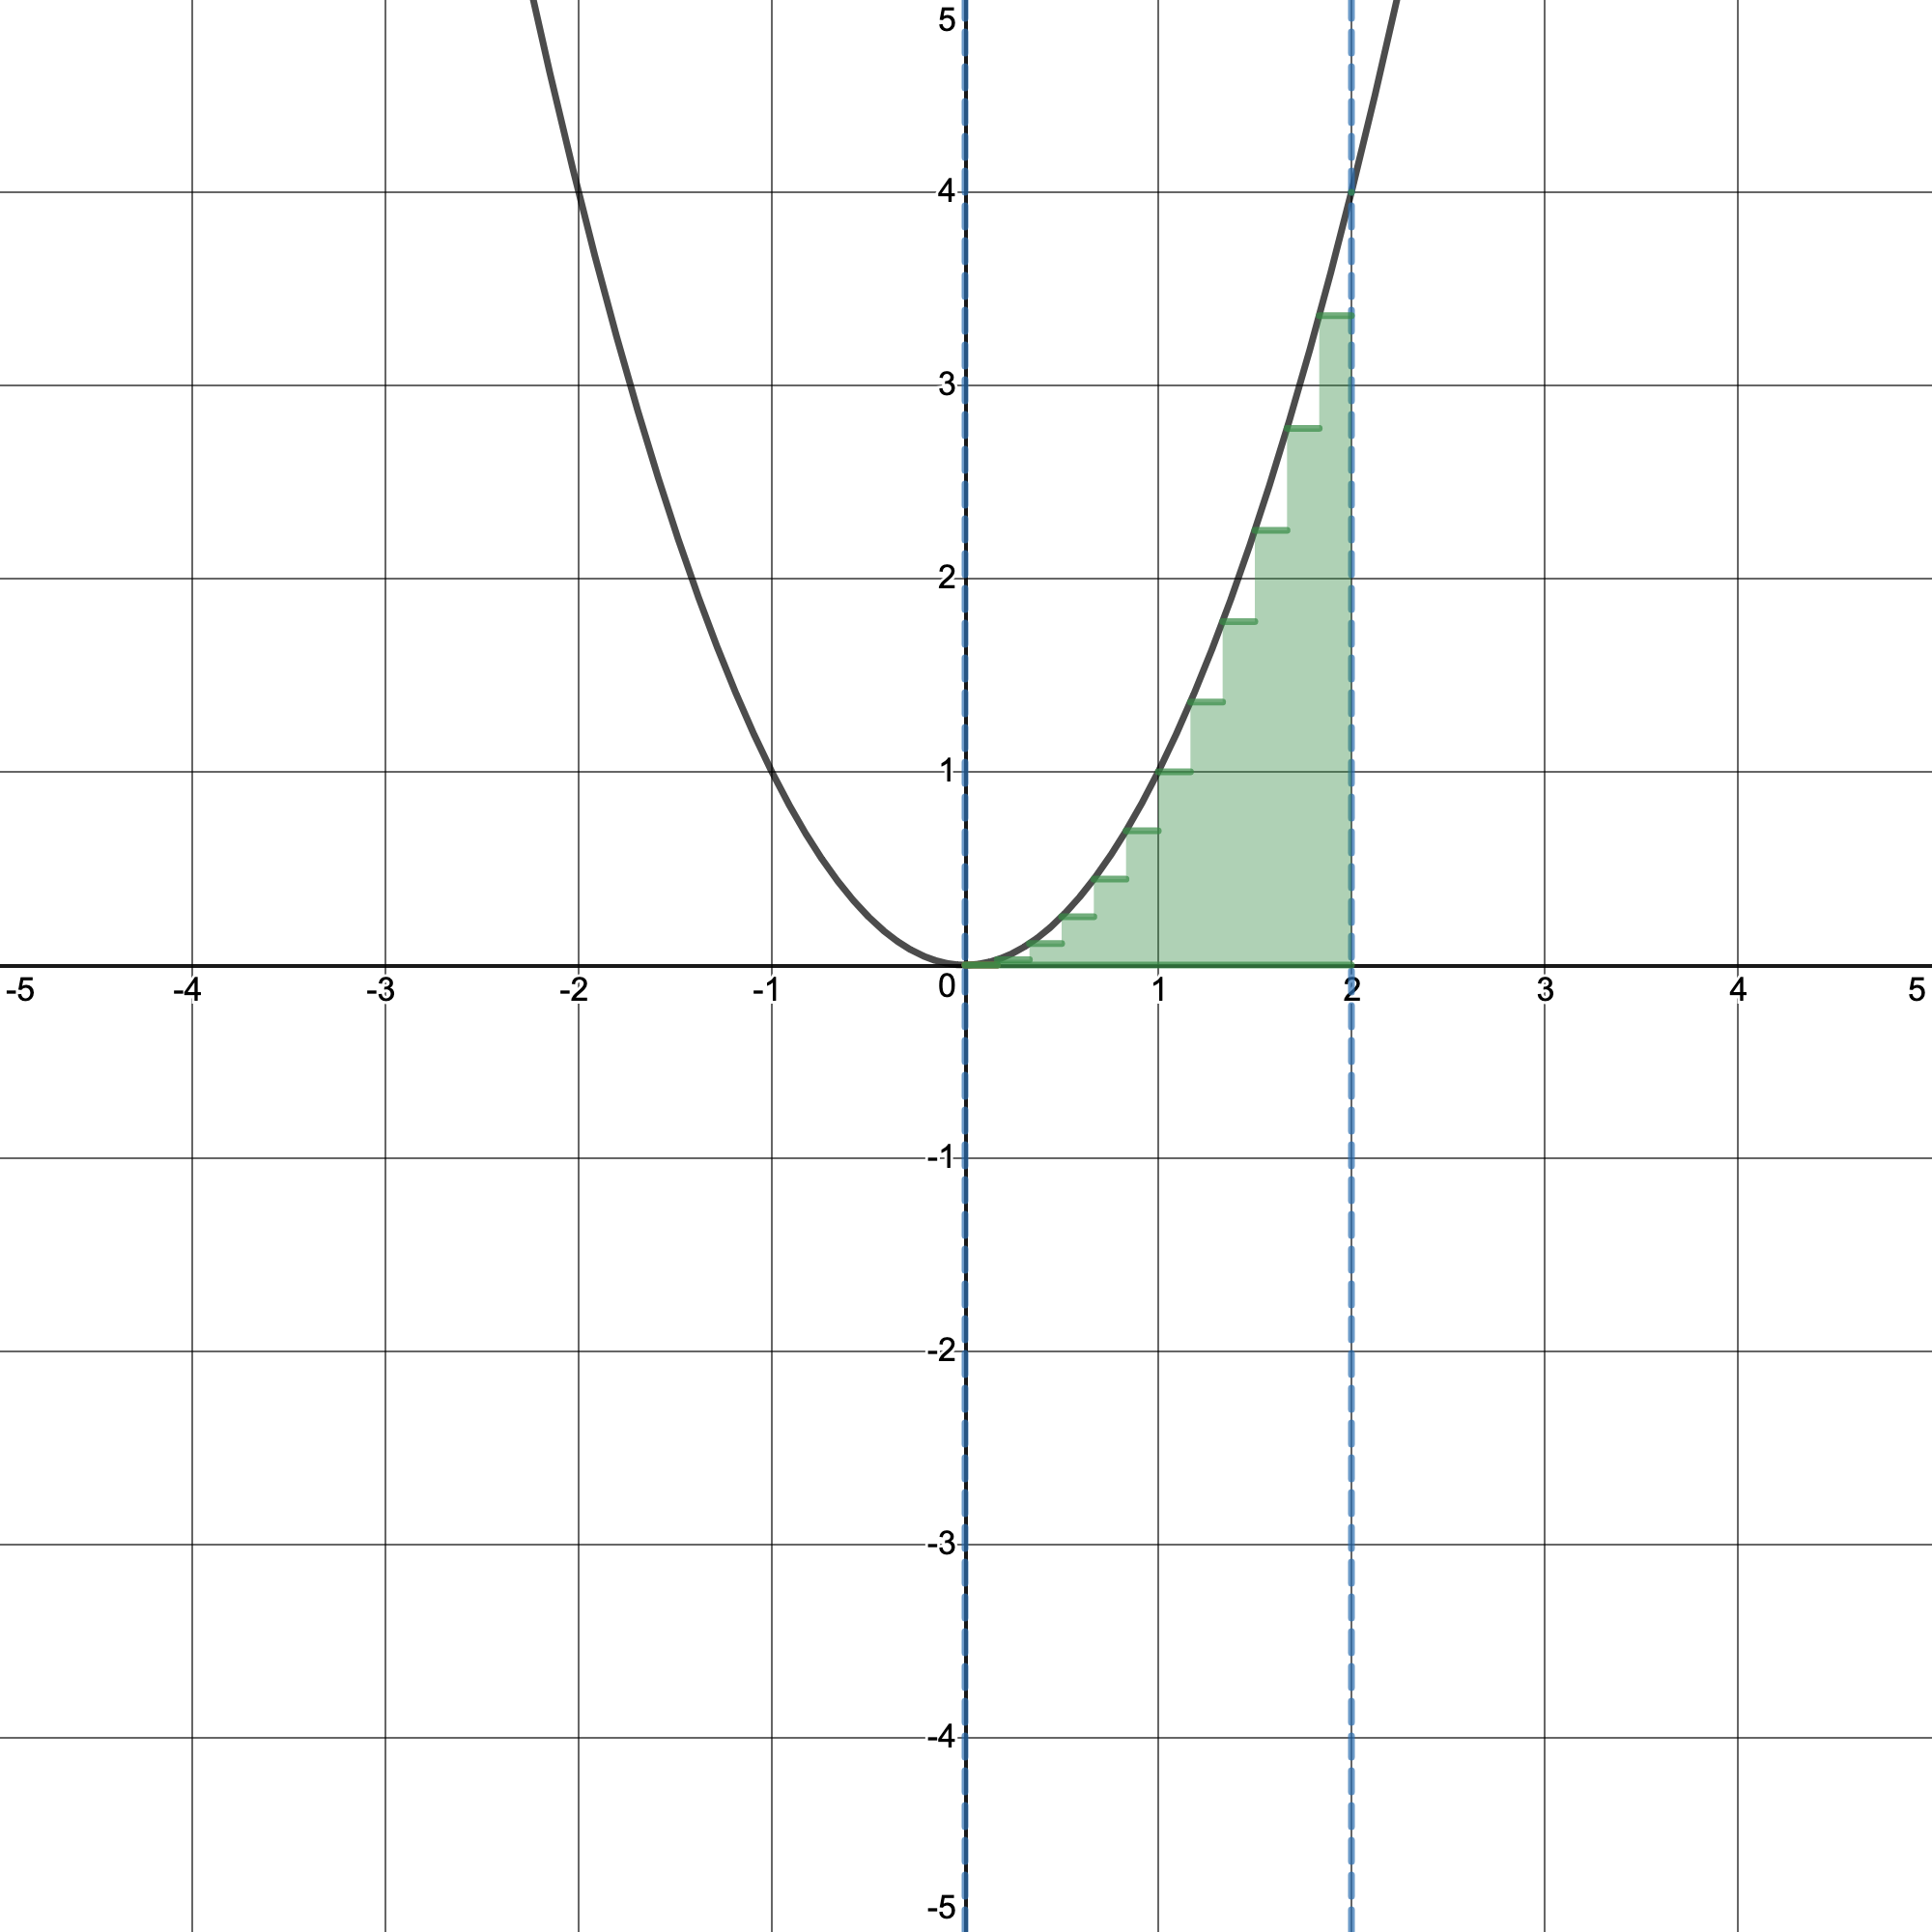
\includegraphics[width=\linewidth]{Blender/Rsum12.png}
        \caption{Twelve subintervals ($n=12$).}
        \label{fig:4b}
    \end{subfigure}
    \caption{Riemann sums for $x^2$.}
    \label{fig:4}
\end{figure}


So what is the best course of action to integrate a, as is the title of Section 2, "Nonintegrable Function?" Of course, there is a hitch --- "Nonintegrable" simply means that it cannot be \emph{perfectly} integrated (integrated via algebraic means) to find another function that exactly describes the area under the initial integrable function at every point. Any function (not at infinity) will have a finite area between itself, the $x$-axis, and the bounds of the integral (generally, $a$ and $b$). Even if this area cannot be expressed in a "pretty" answer in simplest radical form or somesuch, it can be \emph{approximated}. One person could say an area is roughly 2 (for example). Another person could argue that it's 2.2. A third person could say it's 2.17. And as better and better approximations are found, eventually, an approximation can be found that is accurate enough that it suits any real purposes.\par
In fact, all of integration is based on approximations, and then theorems. Integration begins as a Riemann sum, which imagines many small rectangles under a function (see Figure \ref{fig:4} for such rectangles under a parabola). Rectangles are easy to find the area for (just width times height). Let's find the area of the rectangles in Figure \ref{fig:4a}, where there are four rectangles under the parabola, $x^2$. The two vertical, blue-dashed lines are the bounds ($a=0$ and $b=2$ in both subfigures). The width ($w$) of each rectangle can be visually confirmed to be constant and 0.5. Note that the width of one rectangle is also equal to the length of the bounded region divided amont the number of rectangles. Mathematically,
\begin{equation}
    w=\frac{b-a}{n}
\end{equation}
The height of the rectangles is equal to $f(x)$ (where $f(x)=x^2$) at different points. Now, we have the information necessary to write a Riemann sum (the sum of these rectangles' areas; designated $A_a$ for area of Figure \ref{fig:4a}).
\begin{equation*}
    A_a = h_1w_1+h_2w_2+h_3w_3+h_4w_4
\end{equation*}
However, since all of the width's are the same, factor them out and rewrite as just $w$.
\begin{equation*}
    A_a = w(h_1+h_2+h_3+h_4)
\end{equation*}
Substitute in numbers and simplify.
\begin{align*}
    A_a &= 0.5(0+0.25+1+2.25)\\
    &= 1.75
\end{align*}
Is this an approximation? Absolutely. However, more accurate ones may be found. If we sum up the area of all of the rectangles in Figure \ref{fig:4b} (designated $A_b$; this exact process will not be listed, but it's identical to that used to find $A_a$) the area can be found to be about $A_b=2.34$. At this point, the Riemann sum has yielded accuracy to the ones place (note that the exact area is $\frac{8}{3}\approx 2.67$, which can be confirmed by evaluating $\int_0^2 x^2\, dx$).\par
What can we learn from this? We can learn that integrals can be approximated by finding areas via Riemann sums. As you approach infinitely many, infinitely small rectangles, you will approach the exact area and integral. Nothing about a Riemann sum uses antiderivatives (the technique used in Examples 1-15), and it is not as clean, but it does work.\par
To finish this example, let's apply a Riemann sum of $n=4$ on $\left[0,\sqrt{\pi}\right]$ to $\sin(x^2)$, as seen in Figure \ref{fig:5}.\par

\begin{figure}[h!]
    \centering
    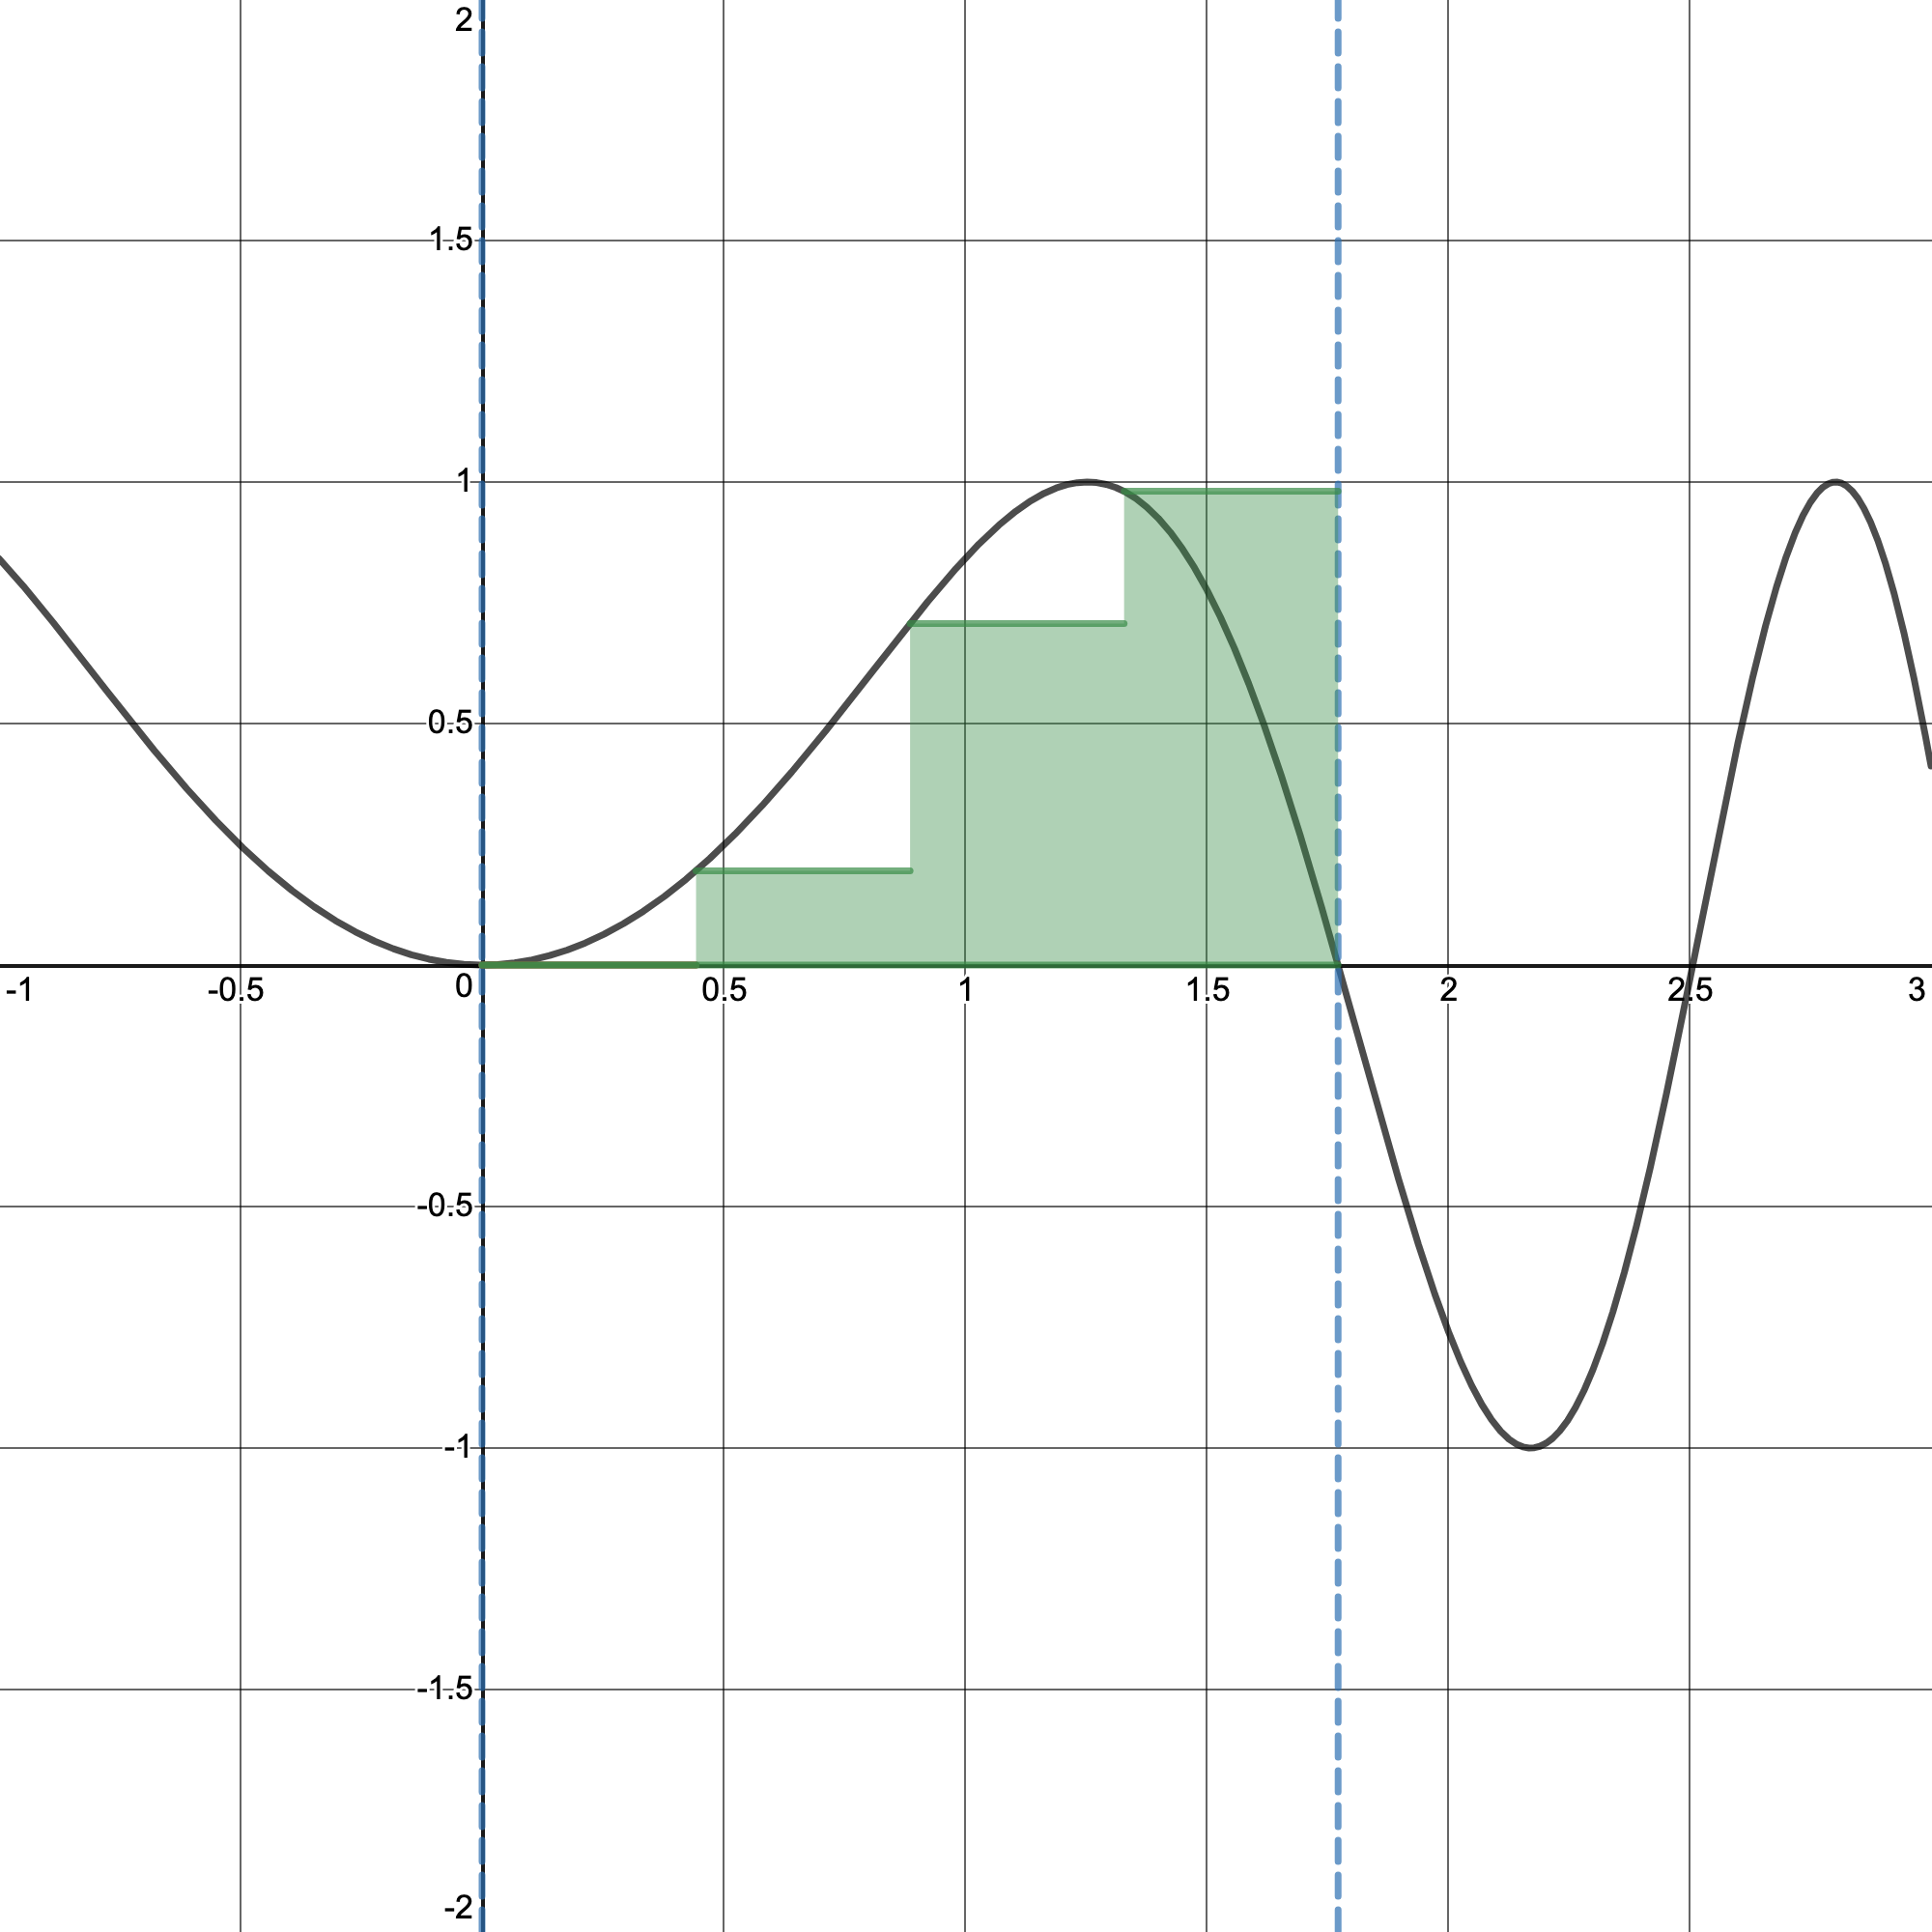
\includegraphics[width=0.4\linewidth]{Blender/Rsum4-sin.png}
    \caption{Riemann sum ($n=4$) for $\sin(x^2)$.}
    \label{fig:5}
\end{figure}

Note that the interval chosen was chosen because it reflects the first positive part of the wave after the $y$-axis. $\sqrt{\pi}$ can be confirmed to be a zero by using arcsine to solve for $x$ in $\sin(x^2)$. However, this will not be proved here.\par
Let's begin summing. Find $w$ by employing equation 26.
\begin{align*}
    w &= \frac{\sqrt{\pi}-0}{12}\\
    &= \frac{\sqrt{\pi}}{12}
\end{align*}
Finding the many values of $h$ has been discussed before, and since the values will not be able to be expressed in simplest radical form due to the nature of the sine function, the summation process will not be shown, but the following, final sum is displayed below (equation 27). Note that both Figures \ref{fig:4} and \ref{fig:5} have used left-hand Riemann sums, which means that after finding $h$, the rectangle is imagined stretching to the right. In Figure \ref{fig:4}, this meant that the rectangles stayed strictly under the function and our estimate was lower. However, since Figure \ref{fig:5} has a descending portion, some of the area approximated by the rectangles sticks outside of the function. This may lead this estimate to be a little more accurate as the excess area will fill in some or all of the area not accounted for by rectangles closer to $x=0$.
\begin{equation}
    A=0.83
\end{equation}
\ex This example is similarly concerned with integrating the following function.$$y=\sin(x^2)$$
There are other techniques which converge to the actual value far faster than Riemann sums. The technique that will be explored in this example is called a Taylor series$^[$\footnote{A calculus-derived polynomial of infinite degree that converges to the values of some function across an interval or over the real numbers, $\mathbb{R}$. The derivation is based off of constructing a polynomial to have the same $n^\text{th}$ derivative as the function in question.}$^]$. Taylor series' can be centered$^[$\footnote{A Taylor series' center is where it most accurately reflects the function in question. The farther away from the center, the less accurate the representation of the function.}$^]$ at different values. For the purposes of this approximation, we'll center at $x=0$, which will also make our Taylor series a Maclaurin series$^[$\footnote{A Maclaurin series is a Taylor series centered at $x=0$.}$^]$.\par
Let's begin deriving a Taylor series. Make a table of the derivatives of $\sin(x^2)$ and their values at $x=0$ (Table \ref{tab:2}).

\begin{table}[h!]
    \centering
    \begin{tabular}{|c|c|c|}
        \hline
        \textbf{Derivative Number} & \textbf{Function} & \textbf{Value at }$\mathbf{x=0}$\\
        \hline
        0 & $\sin(x^2)$ & 0\\
        \hline
        1 & $2x\cos(x^2)$ & 0\\
        \hline
        2 & $2\cos(x^2)-4x^2\sin(x^2)$ & 2\\
        \hline
        3 & $-12x\sin(x^2)-8x^3\cos(x^2)$ & 0\\
        \hline
        4 & $(16x^4-12)\sin(x^2)-48x^2\cos(x^2)$ & 0\\
        \hline
        5 & $160x^3\sin(x^2)+(32x^5-120x)\cos(x^2)$ & 0\\
        \hline
        6 & $(720x^2-64x^6)\sin(x^2)+(480x^4-120)\cos(x^2)$ & $-120$\\
        \hline
    \end{tabular}
    \caption{Derivatives of $\sin(x^2)$.}
    \label{tab:2}
\end{table}

This table could go on forever, but we will curtail it at derivative number 6 since Section 2.1 is all about \emph{restricted} estimates. By finding more and more derivatives, more and more accuracy for more and more values can be achieved. Before we can begin constructing a polynomial to these specifications, let's investigate some calculus properties of polynomials. This will be done in a theorem-proof$^[$\footnote{These will not be formal, deductive proofs, but rather examples from which the theorem will be inferred to hold.}$^]$ fashion, and these theorems will be useful when constructing the Taylor series.\par
\subparagraph{Theorem 1} The value of the $n^\text{th}$ derivative of a polynomial evaluated at $x=0$ is based solely on that polynomial's $n^\text{th}$ degree term.
\subparagraph{Justification} Let's take the polynomial $k_3x^3+k_2x^2+k_1x+k_0$, where all $k$ values are constants. This polynomial could also be written as $$0x^n+0x^{n-1}+\ldots+0x^4+k_3x^3+k_2x^2+k_1x^1+k_0x^0$$This is the version that we will consider. Let's take the zeroeth derivative, i.e. the function as is evaluated at $x=0$. This can easily be confirmed to be $k_0$ as $0^n$ is zero except when $n=0$ and $0^0$ becomes 1.\par
Let's find the first derivative. By the power rule, the first derivative is$$0nx^{n-1}+0(n-1)x^{n-2}+\ldots+0(4)x^3+3k_3x^2+2k_2x^1+1k_1x^0+0$$Note that $0n$, $0(n-1)$, and $0(4)$ are all equal to 0. Evaluating this first derivative at $x=0$ yields $k_1$.\par
Let's find the second derivative. By the power rule, the second derivative is$$0n(n-1)x^{n-2}+0(n-1)(n-2)x^{n-3}+\ldots+0(4)(3)x^2+3(2)k_3x^1+2(1)k_2x^0+0+0$$Note that, similar to last time, many coefficients simplify. Evaluating this second derivative at $x=0$ yields $2k_2$.\par
At this point, a pattern should be emerging. With each successive derivative, the constant (the only thing that shows up at $x=0$) becomes zero, the $x^1$ term's coefficient becomes the constant, and each term is raised to an exponent 1 less in value than before. Through the progression shown (and an imaginary future progression), it can be seen that the $n^\text{th}$ derivative at $x=0$ is indeed dependent on only the $x^n$ term.
\subparagraph{Theorem 2} The value of the $n^\text{th}$ derivative of a polynomial evaluated at $x=0$ can be found through analysis of the $n^\text{th}$ degree term. Furthermore, this value is equal to $n!k$, where $k$ is the coefficient of the $n^\text{th}$ term in the undifferentiated polynomial.
\subparagraph{Justification} Consider a single term in a polynomial. Every time a derivative is taken, the power rule mandates that
\begin{equation*}
    \frac{d}{dx}(kx^n)=nkx^{n-1}
\end{equation*}
As higher derivatives are taken, this process will continue.
\begin{equation*}
    \frac{d}{dx}(nkx^{n-1})=n(n-1)kx^{n-2}
\end{equation*}
The process will go on and on until the exponent reaches the value of zero, at which point the coefficient is just a constant which converts to zero at the next higher derivative. However, this constant \emph{is} predictable based on the initial term. The coefficient, at each higher derivative, will be the initial constant multiplied by $n$, multiplied by the integer one less than $n$, multiplied by the integer two less than $n$, and on and on. If we're looking for the $i^\text{th}$ derivative, the coefficient of the $n^\text{th}$ term is given by
\begin{equation*}
    \frac{n!k}{(n-i)!}
\end{equation*}
By using factorial notation, we have compressed $n(n-1)(n-2)(\ldots)$ into a concise expression. However, to find the value of the $n^\text{th}$ derivative, $i=n$, so the denominator becomes $(n-n)!=0!=1$, and the overall expression for the $n^\text{th}$ derivative condenses to the following.
\begin{equation*}
    n!k
\end{equation*}
\subparagraph{Theorem 3} The $x^n$ term in a polynomial with the $n^\text{th}$ derivative $c$ when evaluated at $x=0$ will have a coefficient of $\frac{c}{n!}$.
\subparagraph{Justification} This follows fairly directly from Theorem 2. Theorem 2 states that if the $n^\text{th}$ term is $kx^n$, the $n^\text{th}$ derivative at $x=0$ will be $n!k$. If we need to find $k$ in terms of $c$, set $c$ equal to the known value of the $n^\text{th}$ derivative and solve.
\begin{align*}
    n!k &= c\\
    k &= \frac{c}{n!}
\end{align*}\par
\bigskip
The first two theorems were mainly to build up to Theorem 3, which will be used here to construct the Taylor series. We will also finally need Table \ref{tab:2}. In the context of Theorem 3, the right column of Table \ref{tab:2} provides a list of $n^\text{th}$ derivatives, $c$, for which we must find a $k$ value. Table \ref{tab:2} goes up to the $6^\text{th}$ derivative, so this Taylor polynomial will be sixth degree. Note that Taylor series (polynomials) are written with their terms ordered by ascending degree as opposed to descending (because a full Taylor series would have an $x^\infty$ term.\par
Write a sixth degree polynomial with variable coefficients.
\begin{equation*}
    c_0+c_1x+c_2x^2+c_3x^3+c_4x^4+c_5x^5+c_6x^6
\end{equation*}
By Theorem 3, $c_n=\frac{k_n}{n!}$. Substitute.
\begin{equation*}
    \frac{k_0}{0!}+\frac{k_1}{1!}x+\frac{k_2}{2!}x^2+\frac{k_3}{3!}x^3+\frac{k_4}{4!}x^4+\frac{k_5}{5!}x^5+\frac{k_6}{6!}x^6
\end{equation*}
Simplify.
\begin{equation*}
    k_0+k_1x+\frac{k_2}{2}x^2+\frac{k_3}{6}x^3+\frac{k_4}{24}x^4+\frac{k_5}{120}x^5+\frac{k_6}{720}x^6
\end{equation*}
Substitute in all values from the right column of Table \ref{tab:2} for their corresponding $k$ value.
\begin{equation*}
    0+0x+\frac{2}{2}x^2+\frac{0}{6}x^3+\frac{0}{24}x^4+\frac{0}{120}x^5+\frac{-120}{720}x^6
\end{equation*}
Simplify.
\begin{equation}
    x^2-\frac{1}{6}x^6
\end{equation}
Let's evaluate how close this polynomial is to the original function. Figure \ref{fig:6} shows three graphs of the function with $y=0$, $y=x^2$, and all of equation 28 overlain.

\begin{figure}[h!]
    \centering
    \begin{subfigure}[b]{0.3\linewidth}
        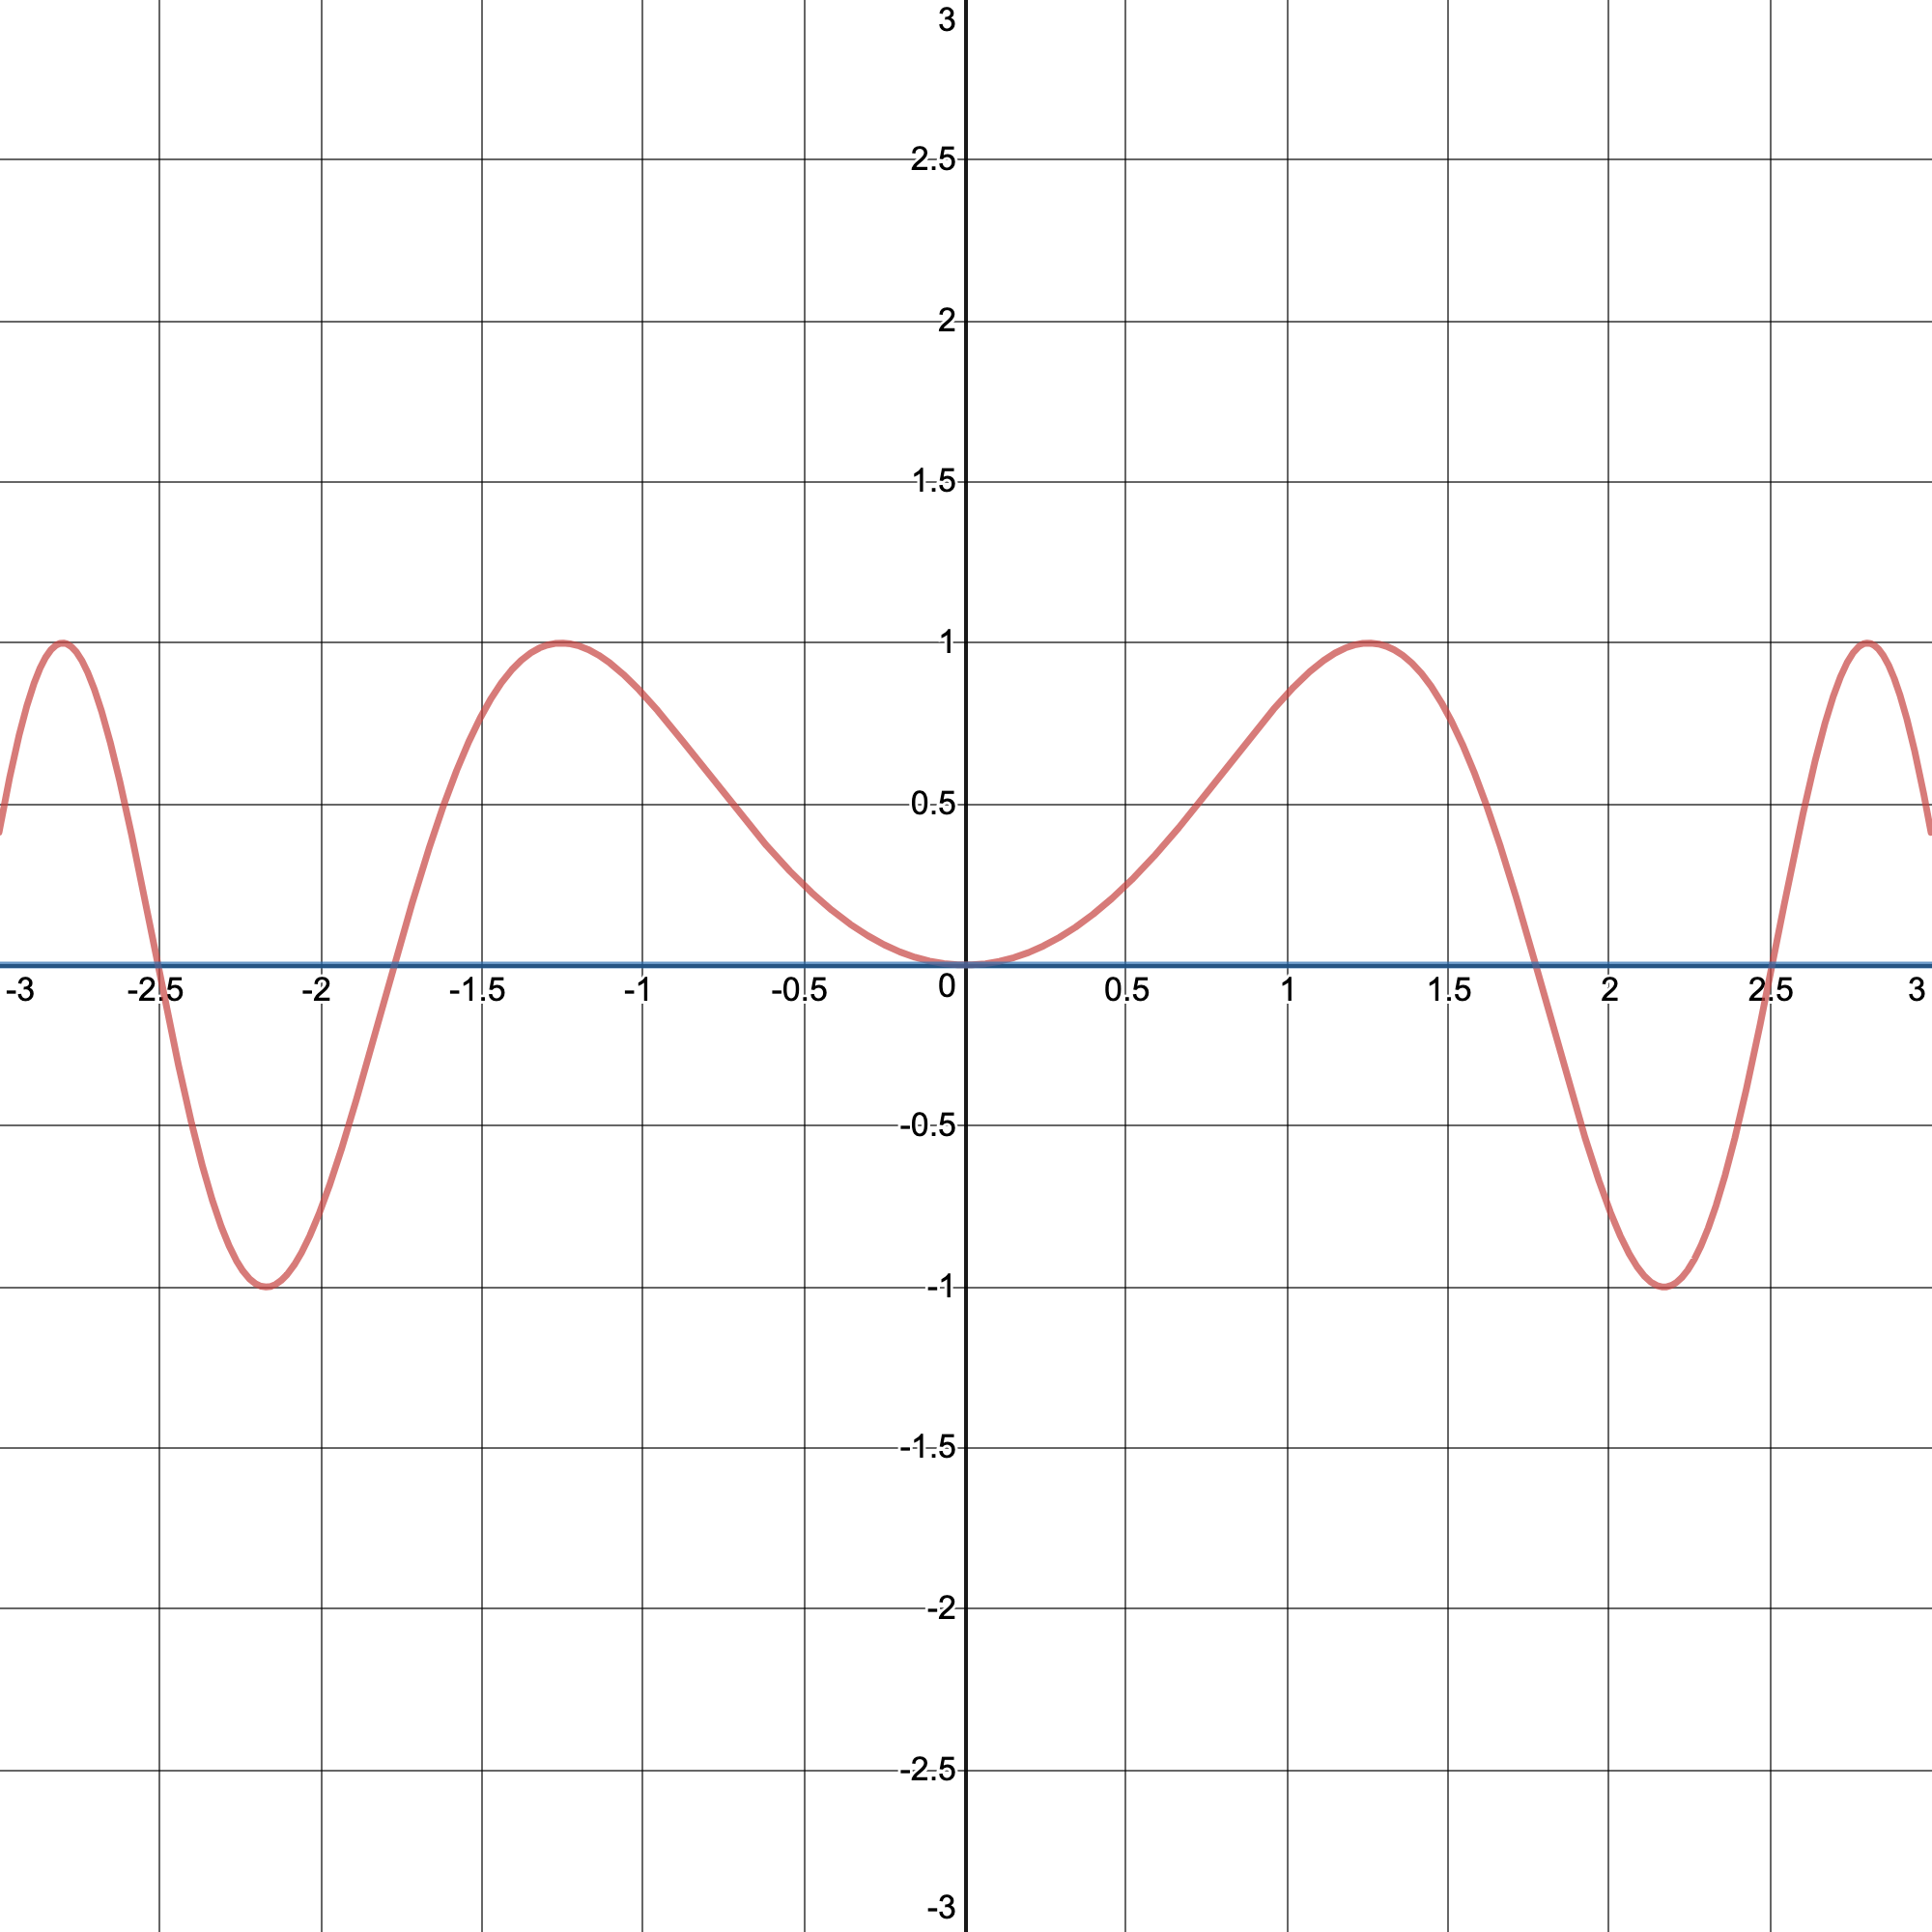
\includegraphics[width=\linewidth]{Blender/y-0.png}
        \caption{$\sin(x^2)$ versus $y=0$.}
        \label{fig:6a}
    \end{subfigure}\hspace{1.5em}
    \begin{subfigure}[b]{0.3\linewidth}
        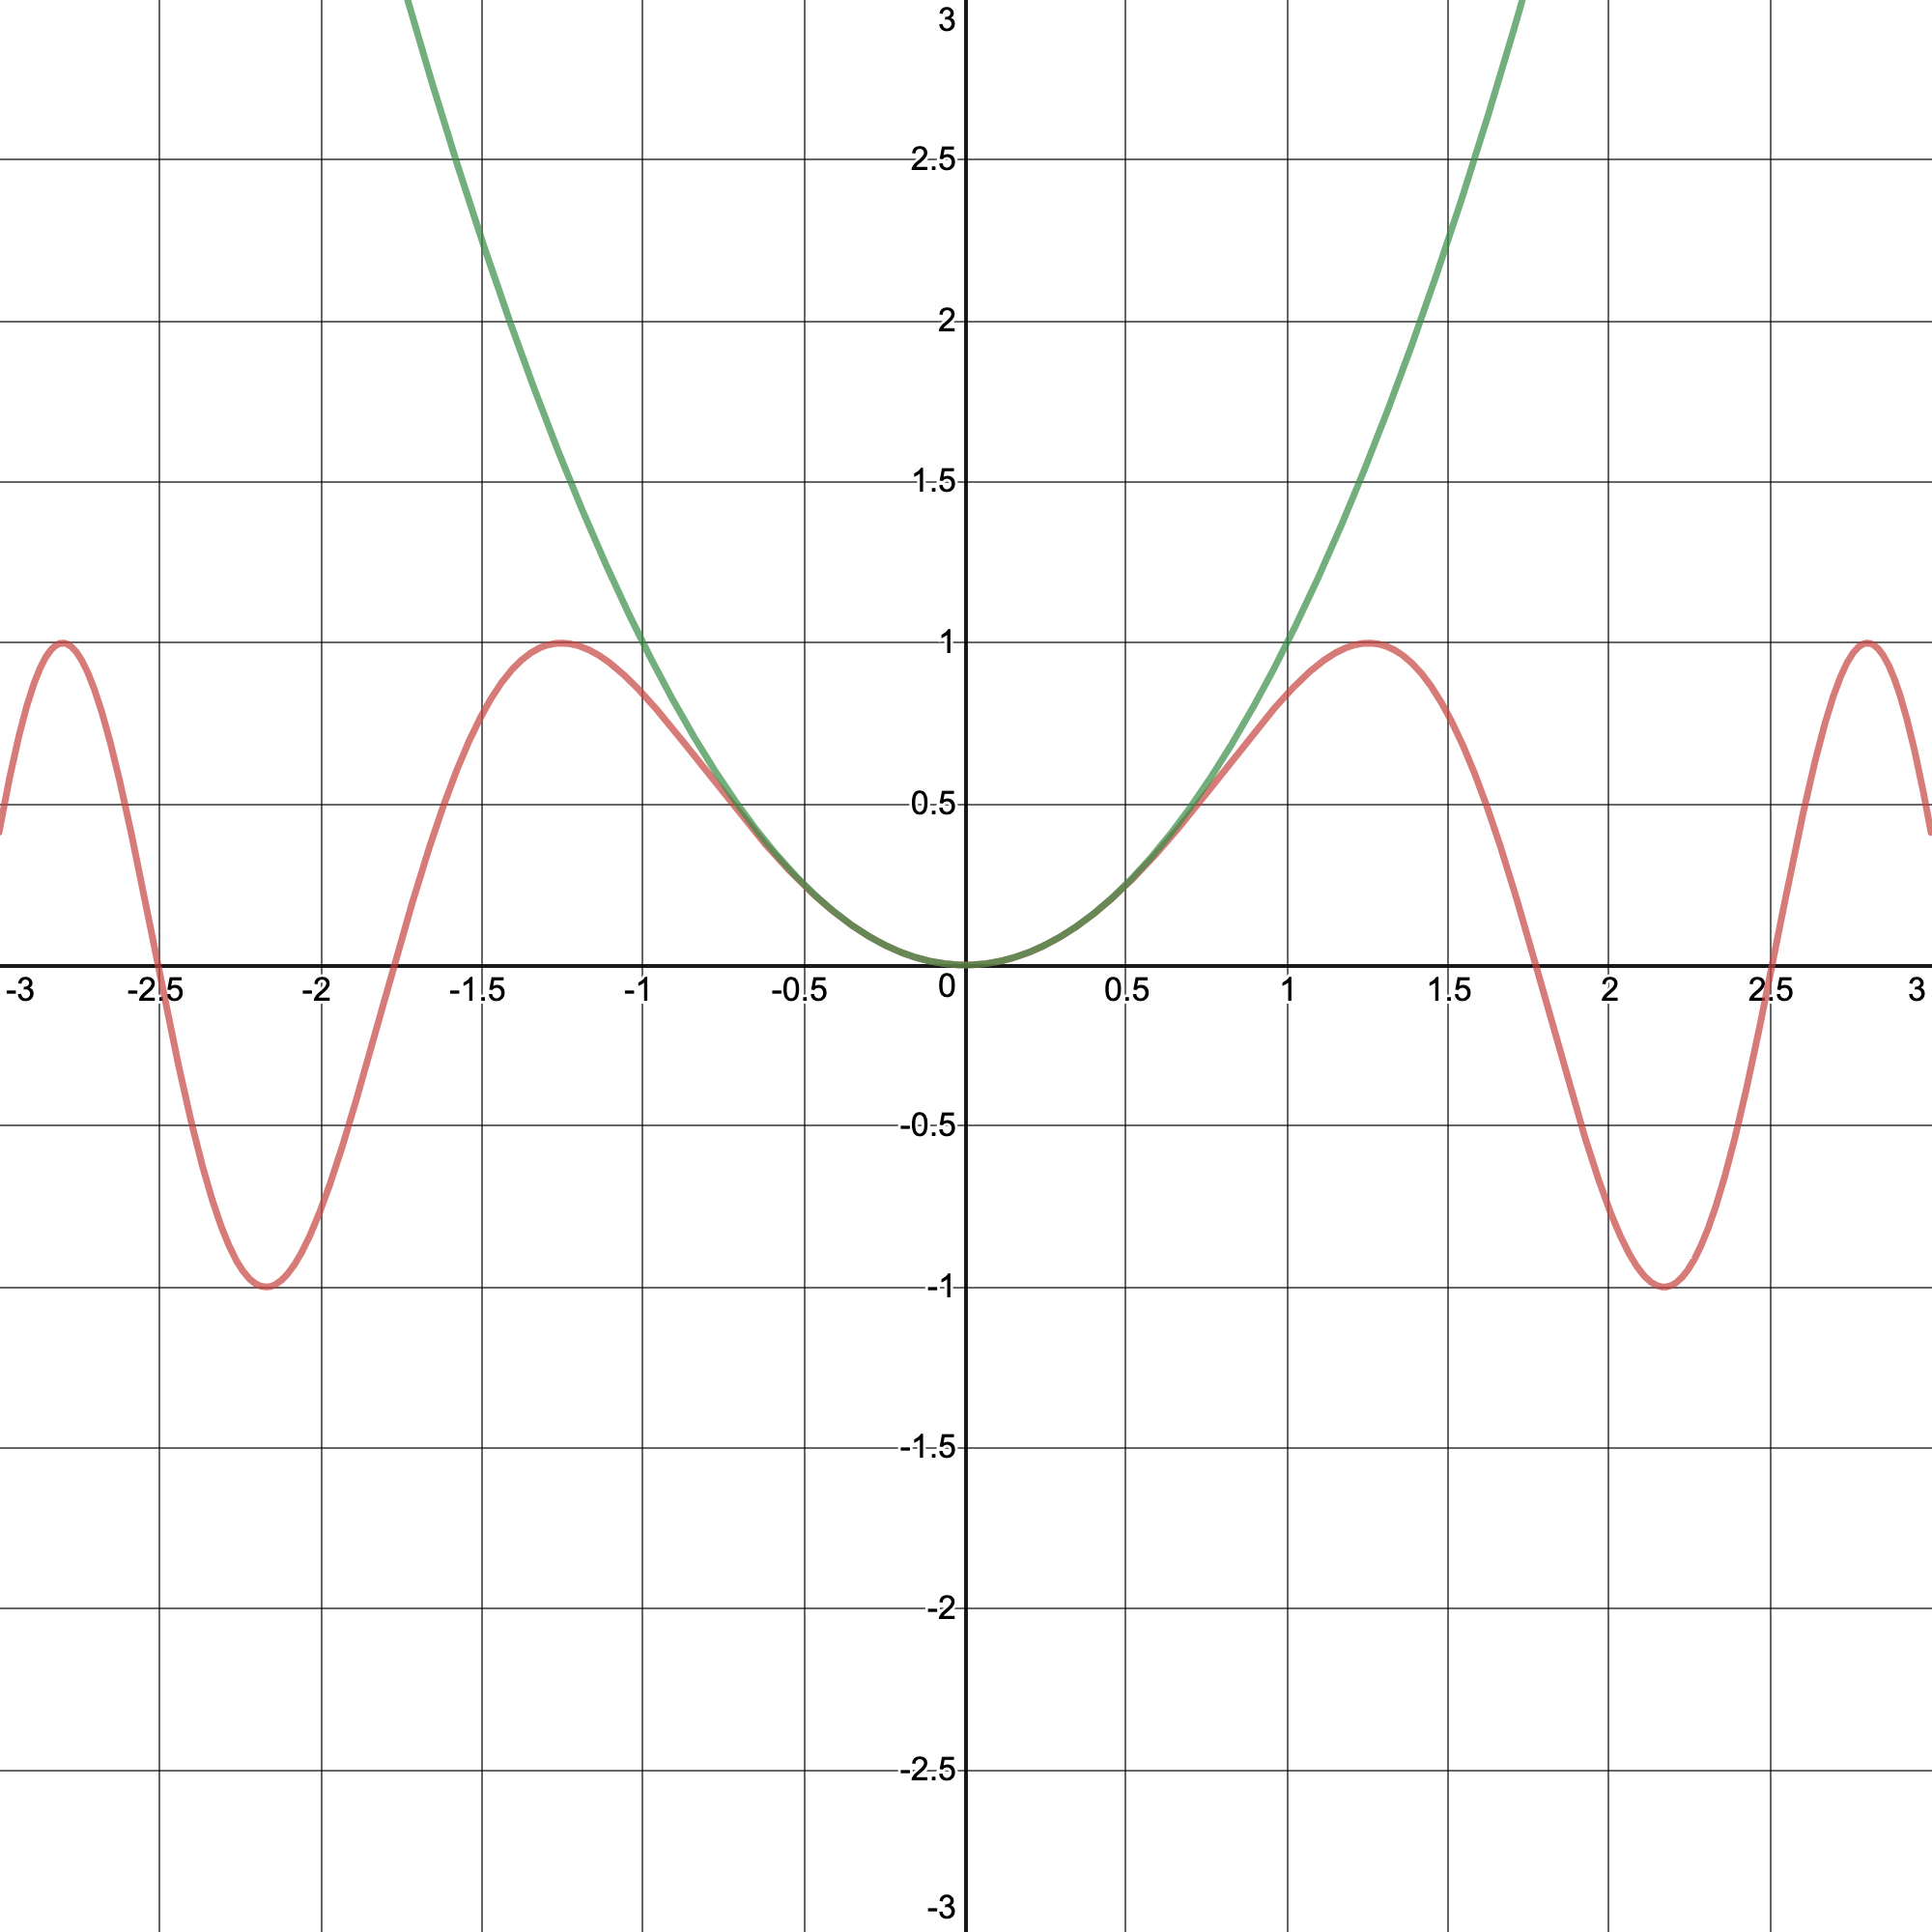
\includegraphics[width=\linewidth]{Blender/y-x2.png}
        \caption{$\sin(x^2)$ versus $y=x^2$.}
        \label{fig:6b}
    \end{subfigure}\hspace{1.5em}
    \begin{subfigure}[b]{0.3\linewidth}
        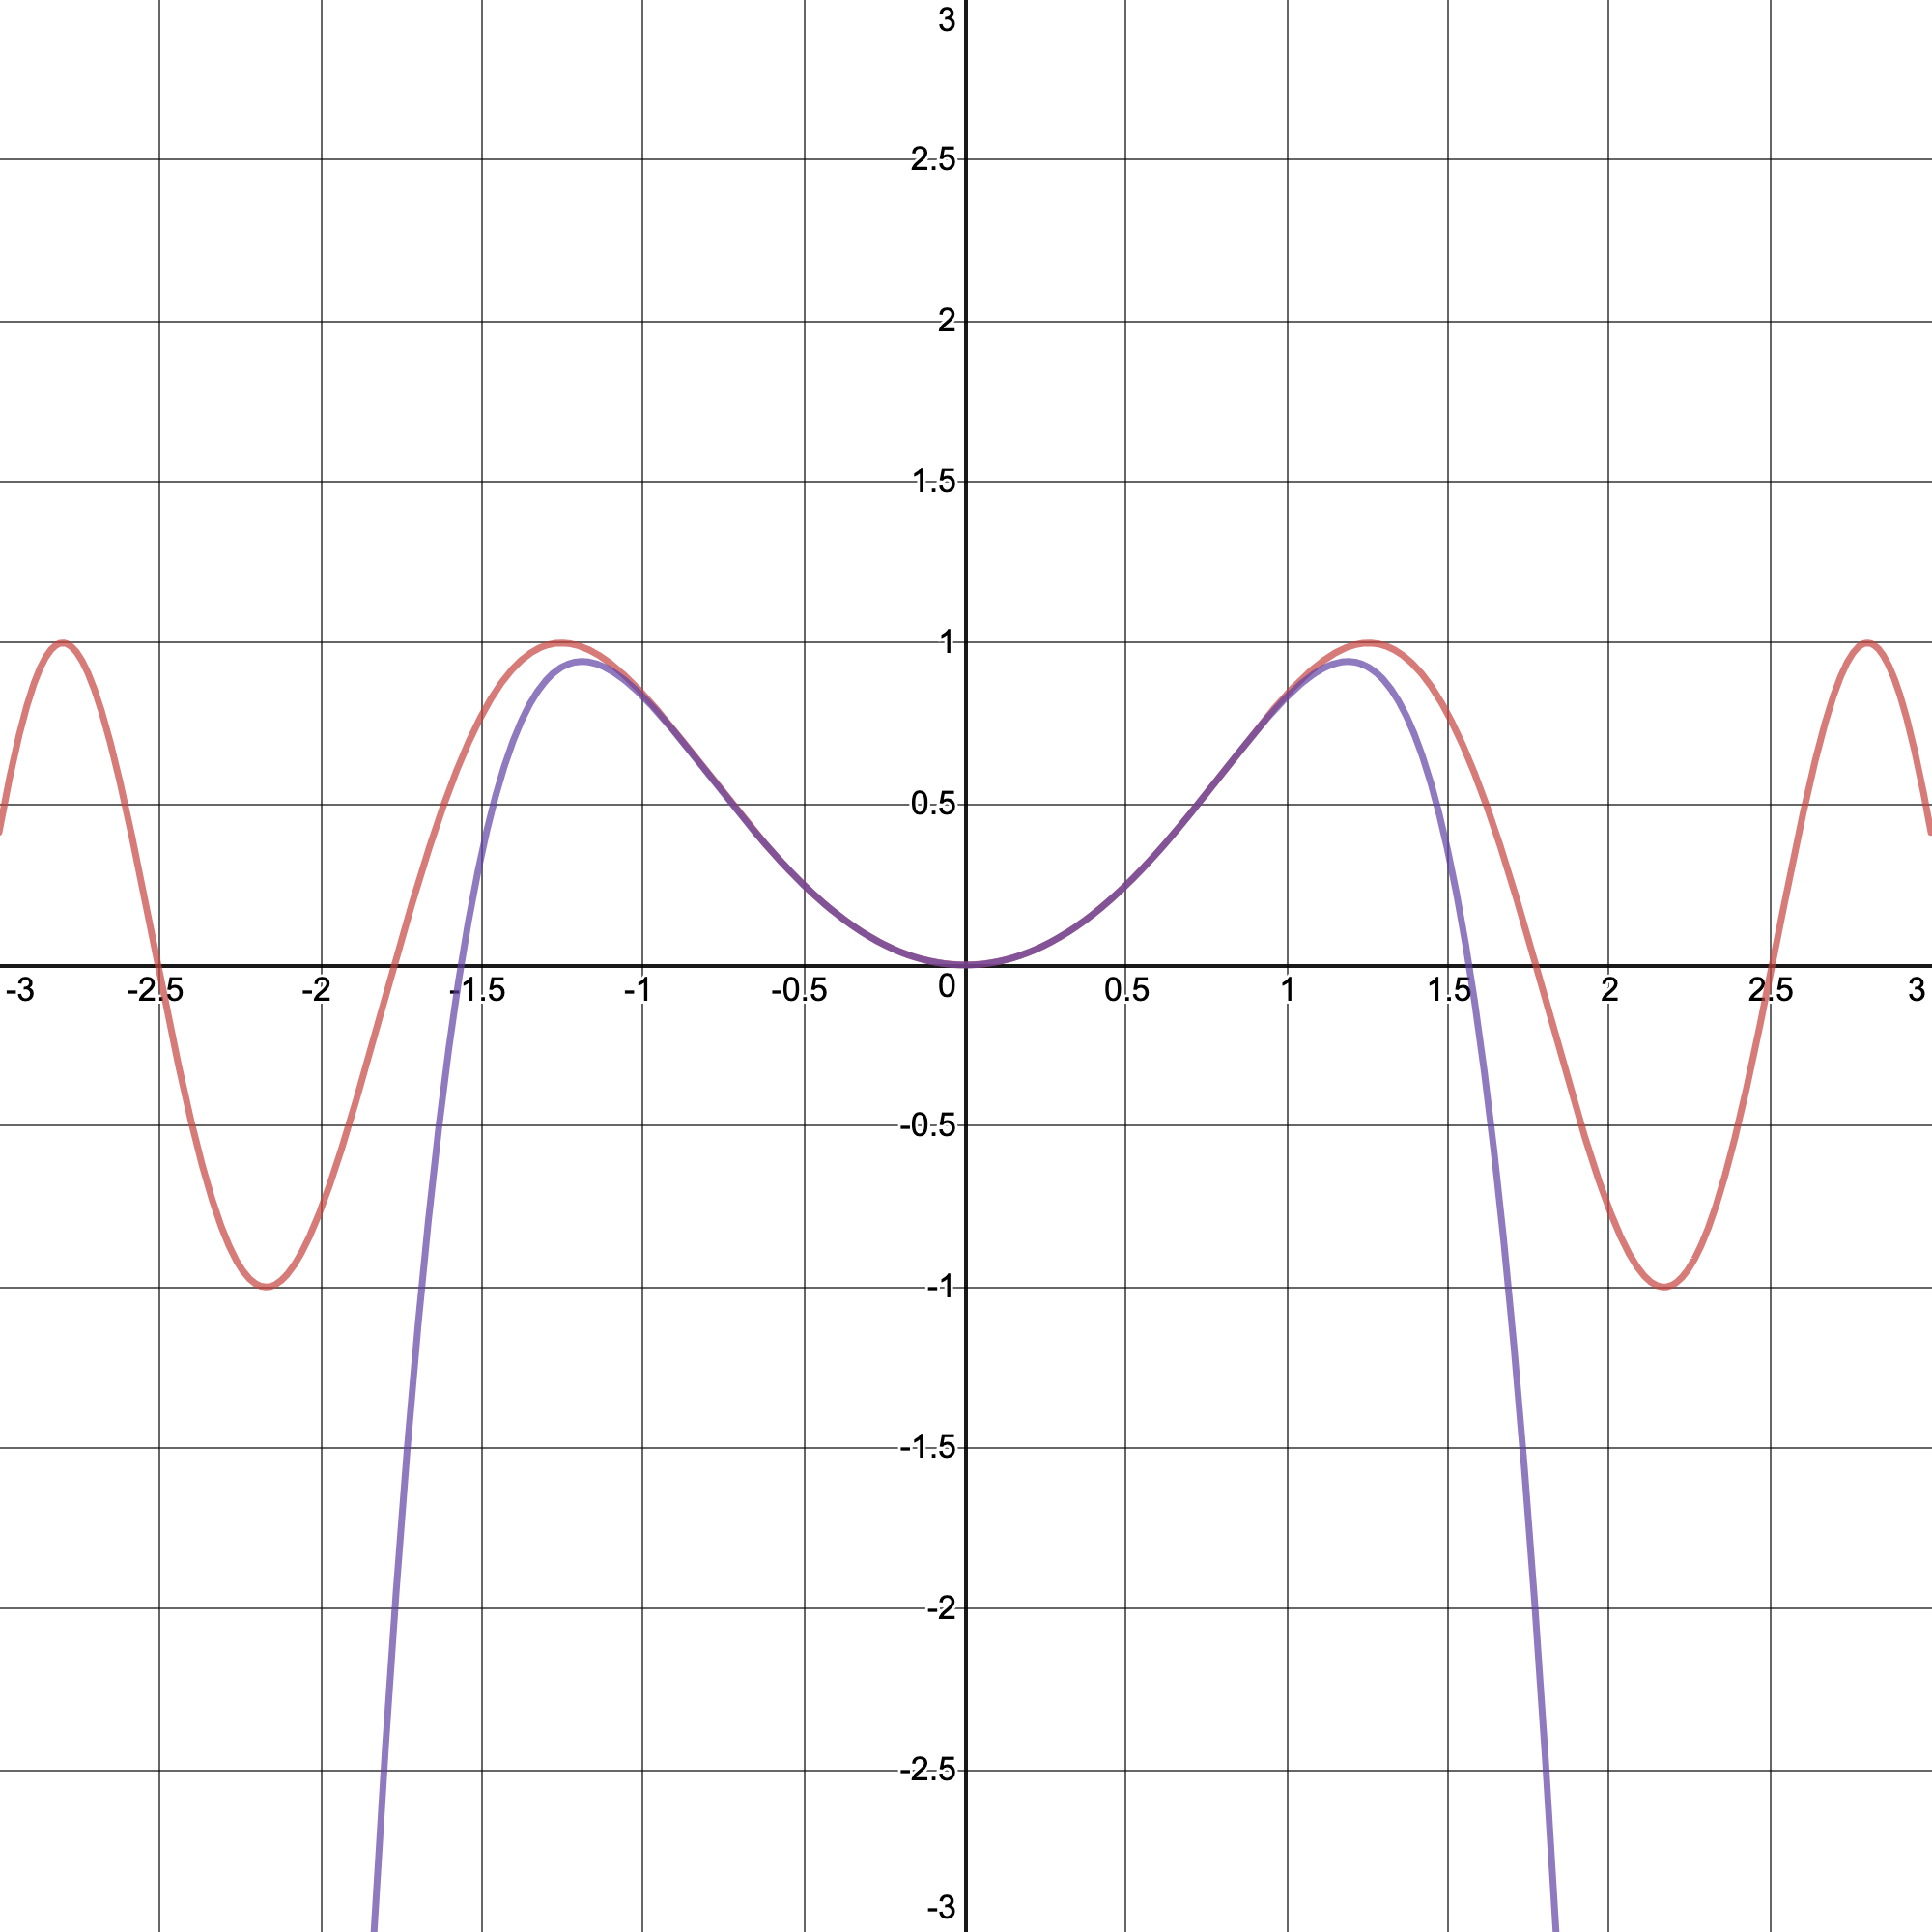
\includegraphics[width=\linewidth]{Blender/y-28.png}
        \caption{$\sin(x^2)$ versus equation 28.}
        \label{fig:6c}
    \end{subfigure}
    \caption{Three levels of accuracy in approximating $\sin(x^2)$ by Taylor series.}
    \label{fig:6}
\end{figure}

Similar to Example 16, a Taylor series is better at finding area (definite integrals) than indefinite integrals, though it is possible to achieve a decent one over a range with a great deal of terms. The key to using a Taylor series for definite integrals is that it is a polynomial which approximates the behavior of the function in question, and a polynomial can be easily integrated via the antipower rule between $a$ and $b$. This integral is the approximation. Finding more accuracy requires finding more terms in the Taylor series, as opposed to using more rectangles as with the Riemann sum. However, finding the indefinite integral of the Taylor series will give an approximation of the indefinite integral of the function, as well.\par
Let's integrate the Taylor series on $\left[0,\sqrt{\pi}\right]$. To be comparable to the Riemann sum in Example 16, I continued the Taylor series to 4 terms. Write the integrable equation as follows.
\begin{equation*}
    A=\int_0^{\sqrt{\pi}} \left(x^2-\frac{1}{6}x^6+\frac{1}{120}x^{10}-\frac{1}{5040}x^{14}\right)\, dx
\end{equation*}
Evaluate this using the techniques discussed in Example 1. This process will not be displayed here. However, it yields the following, final sum which is displayed below (equation 29). It should be noted that this answer is accurate to two decimal places whereas the Riemann sum was only accurate to one (the exact area between $\sin(x^2)$ and the $x$-axis on $\left[0,\sqrt{\pi}\right]$ as an abbreviated decimal is $0.894831\ldots$).
\begin{equation}
    A=0.89
\end{equation}
\paragraph{Summary} Throughout this section, Riemann sums and Taylor series were explored as methods of approximating definite integrals for functions that are not algebraically integrable. Taylor series converge far faster, but also require more setup and a deeper knowledge of calculus. The next section will explore a way of more quickly generating a Taylor series and coming closer to an "exact value" expression as opposed to repeating decimals.
\newpage


\subsection{Sigma Notation}
\paragraph{Introduction} This section contains only one example. The theory of Sigma notation will be developed, followed by an indefinite and definite evaluation of the integrable equation.
\ex This example is concerned with integrating the following function.$$y=\text{e}^{-x^2}$$
A Taylor \emph{series} (as opposed to the Taylor \emph{polynomials} that have been explored) is nothing more than an infinite sum. The derivatives in Table \ref{tab:2} became very messy very quickly, but some functions have Taylor polynomials in which a clear pattern emerges$^[$\footnote{For the purposes of this paper, convergence will be assumed and not proved. Examples are chosen that converge over $\mathbb{R}$.}$^]$.\par
Differentiating $\text{e}^{-x^2}$ could become a difficult task very quickly. However, differentiating the parent function ($\text{e}^x$) could not be simpler. $\text{e}^x$ is its own derivative, so the $n^\text{th}$ derivative of $\text{e}^x$ evaluated at $x=0$ will always be $1$ since $\text{e}^0=1$.\par
Let's begin deriving a Taylor series. To follow a relatable process to Example 17, make a table of the derivatives of $\text{e}^x$ (not $\text{e}^{-x^2}$) and their values at $x=0$ (Table \ref{tab:3}).

\begin{table}[h!]
    \centering
    \begin{tabular}{|c|c|c|}
        \hline
        \textbf{Derivative Number} & \textbf{Function} & \textbf{Value at }$\mathbf{x=0}$\\
        \hline
        0 & $\text{e}^x$ & $1$\\
        \hline
        1 & $\text{e}^x$ & $1$\\
        \hline
        2 & $\text{e}^x$ & $1$\\
        \hline
        3 & $\text{e}^x$ & $1$\\
        \hline
        4 & $\text{e}^x$ & $1$\\
        \hline
        5 & $\text{e}^x$ & $1$\\
        \hline
        6 & $\text{e}^x$ & $1$\\
        \hline
    \end{tabular}
    \caption{Derivatives of $\text{e}^x$.}
    \label{tab:3}
\end{table}

Write a sixth degree polynomial with variable coefficients.
\begin{equation*}
    c_0+c_1x+c_2x^2+c_3x^3+c_4x^4+c_5x^5+c_6x^6
\end{equation*}
By Theorem 3, $c_n=\frac{k_n}{n!}$. Substitute.
\begin{equation}
    \frac{k_0}{0!}+\frac{k_1}{1!}x+\frac{k_2}{2!}x^2+\frac{k_3}{3!}x^3+\frac{k_4}{4!}x^4+\frac{k_5}{5!}x^5+\frac{k_6}{6!}x^6
\end{equation}
Simplify.
\begin{equation*}
    k_0+k_1x+\frac{k_2}{2}x^2+\frac{k_3}{6}x^3+\frac{k_4}{24}x^4+\frac{k_5}{120}x^5+\frac{k_6}{720}x^6
\end{equation*}
Substitute in all values from the right column of Table \ref{tab:3} for their corresponding $k$ value.
\begin{equation*}
    1+1x+\frac{1}{2}x^2+\frac{1}{6}x^3+\frac{1}{24}x^4+\frac{1}{120}x^5+\frac{1}{720}x^6
\end{equation*}
Simplify.
\begin{equation}
    1+x+\frac{x^2}{2}+\frac{x^3}{6}+\frac{x^4}{24}+\frac{x^5}{120}+\frac{x^6}{720}
\end{equation}
At this point, a pattern should be emerging. For starters, the $n^\text{th}$ term clearly has an $x^n$ term. The coefficient may be a little more elusive, but refering to equation 30 reveals it to be $n!$. With these two facts, it is possible to state that the $n^\text{th}$ term will be
\begin{equation*}
    \frac{x^n}{n!}
\end{equation*}
This expression of a term as a function of $n$ makes it possible to compress the equation 31 into Sigma notation$^[$\footnote{Sigma notation (or summation notation) is a method of writing a finite or infinite sum in a concise manner. The argument is a function of a variable that progresses from $a$ to $b$ among the integers, $\mathbb{Z}$.}$^]$.\par
Let's familliarize ourselves with Sigma notation before tackling equation 31. Consider the following expression.
\begin{equation*}
    \sum_{n=1}^4 n^2
\end{equation*}
There is a lot of information to unpack here. The \textbf{function} is $n^2$. The \textbf{initial value} is $1$. The \textbf{final value} is $4$. To begin expanding this expression, plug in the initial value for $n$.
\begin{equation*}
    \sum_{n=1}^4 n^2 = 1^2\ldots
\end{equation*}
Then, plug in the integer following the initial value for $n$. Add this value to the first term.
\begin{equation*}
    \sum_{n=1}^4 n^2 = 1^2+2^2\ldots
\end{equation*}
The reader may now be able to see where this is going. Add the function of $3$ and the function of $4$. At $4$, we are finished since the final value is equal to $4$.
\begin{equation*}
    \sum_{n=1}^4 n^2 = 1^2+2^2+3^2+4^2
\end{equation*}
In this case, the right side can be simplified.
\begin{equation*}
    \sum_{n=1}^4 n^2 = 30
\end{equation*}
Returning to equation 31, substitute in the generalized $n^\text{th}$ term that follows it, change the initial value to 0, and change the final value to 6. 
\begin{equation*}
    \sum_{n=0}^6 \frac{x^n}{n!} = 1+x+\frac{x^2}{2}+\frac{x^3}{6}+\frac{x^4}{24}+\frac{x^5}{120}+\frac{x^6}{720}
\end{equation*}
The left side of the above equation can be confirmed to be equal to the right side (this will be left as an exercise to the reader). By using Sigma notation, a sixth degree Taylor polynomial has been compressed into a tidy package. Furthermore, to make signify a higher degree Taylor polynomial only requires increasing the final value in the expression. In fact, sigma notation makes it feasible to convey an infinite series, which is directly equivalent to $\text{e}^x$.
\begin{equation*}
    \sum_{n=0}^\infty \frac{x^n}{n!} = \text{e}^x
\end{equation*}\par
\bigskip
Now, how does all of this relate to $\text{e}^{-x^2}$? The answer lies in Example 4. To reiterate, the choice of $x$ as a variable is arbitrary. As long as it is used consistently, any letter can be chosen. For example, $u$.
\begin{equation*}
    \sum_{n=0}^\infty \frac{u^n}{n!} = \text{e}^u
\end{equation*}
The above statement is just as true as the statement two above. However, as of right now, $u$ varies over the real numbers, $\mathbb{R}$, from $-\infty$ to $\infty$. If necessary, though, $u$ can vary in a different manner. For example, we could define$$u=-x^2$$As long as this definition is consistently substituted, the statement will remain true. Substitute the above definition of $u$.
\begin{equation*}
    \sum_{n=0}^\infty \frac{(-x^2)^n}{n!} = \text{e}^{-x^2}
\end{equation*}
At this point, we have found an acceptable Sigma notation representation of the Taylor series for $\text{e}^{-x^2}$. However, this is not generally the form in which the statement is displayed, so a few modifications will follow.\par
Employ the rule of exponents that $(ab)^m=a^mb^m$.
\begin{equation*}
    \sum_{n=0}^\infty \frac{(-1)^n(x^2)^n}{n!} = \text{e}^{-x^2}
\end{equation*}
Employ the rule of exponents that $(a^m)^n=a^{mn}$.
\begin{equation*}
    \sum_{n=0}^\infty \frac{(-1)^n(x^{2n})}{n!} = \text{e}^{-x^2}
\end{equation*}
Move the oscillator$^[$\footnote{\emph{Oscillator} is another term for $(-1)^n$. This is a common occurance in Sigma notation for Taylor series because of its ability to oscillate (change) whether the next term is added or subtracted for each successive term.}$^]$ out of the numerator. Note that it is not necessary to add parentheses because all parts are multiplied, but it makes the expression visually easier to parse.
\begin{equation} \label{eq:32}
    \sum_{n=0}^\infty \left((-1)^n\cdot\frac{x^{2n}}{n!}\right) = \text{e}^{-x^2}
\end{equation}
Equation \ref{eq:32} is certainly an important result in the process of integrating $\text{e}^{-x^2}$, but it is not the last step. The left side of equation \ref{eq:32} is only a model of $\text{e}^{-x^2}$, not of its integral. Fortunately, by the antipower rule, integration of a polynomial is a very simple process. To reiterate from Example 1,
\begin{equation*}
    \int x^n = \frac{x^{n+1}}{n+1}
\end{equation*}
In fact, this statement makes integration directly possible within sigma notation. To integrate a polynomial in sigma notation, just integrate $x$ power term as if $n$ is a variable (as done above).
\begin{align*}
    \text{e}^{-x^2} &= \sum_{n=0}^\infty \left((-1)^n\cdot\frac{x^{2n}}{n!}\right)\\
    &\rightarrow \sum_{n=0}^\infty \left((-1)^n\cdot\frac{x^{2n+1}}{n!(2n+1)}\right)+C\tag{33}
\end{align*}
As it so happens, equation 33 does give a representation of the exact indefinite integral other than$$\int \text{e}^{-x^2}\, dx$$That being said, sigma notation also works with definite integrals, as was alluded to earlier. In a strikingly similar fashion to the second part of the Fundamental Theorem of Calculus, the following, final statement can be made (equation 33). Logically, though, it does make sense --- $x$ is just a variable, so its convergence is a function, but a single value will just converge to its antiderivative directly.
\begin{equation}
    \int_a^b \text{e}^{-x^2}\, dx = \sum_{n=0}^\infty \left((-1)^n\cdot\frac{b^{2n+1}}{n!(2n+1)}\right)-\sum_{n=0}^\infty \left((-1)^n\cdot\frac{a^{2n+1}}{n!(2n+1)}\right)
\end{equation}
\paragraph{Summary} Throughout this section, infinite series have been shown to be the solution to every type of one-variable function discussed at the Calculus I-II level. Note that Taylor series would work for any example in this paper, though not every one would compress to Sigma notation as cleanly (or at all).
\newpage



\setcounter{secnumdepth}{0}
\begin{center}
\section{Conclusion}
\end{center}
This paper has explored eighteen wildly different functions of one-variable. A great deal of the examples required ingenious rewrites to transform them to a form that could be integrated by a simpler rule. However, when that failed, there were approximations of difficult functions (Taylor polynomials) and more exact expressions (Taylor series), but still with their own drawbacks.\par
I hope that this paper was enjoyable, informative, and clear.

\vspace{4em}
\noindent All figures are either the designs of the author, created in Blender 3D, or they are exports from Desmos, an online graphing calculator.




\end{document}